%Associate Editor (Remarks to Author): 
%
%The paper presents a methodology for calculating a probabilistic forecast of ash plume dispersion, which is then applied to the Eyjafjallajokull eruption. The topic may be of interest to JAMES readers, but the manuscript requires revision before it can be sent for peer review. 
%
%Specifically, the authors must address the following points. 
%
%1. The descriptions of the models and methods needs to be streamlined. Please revise the description to be succinct and explain the setup of the model runs clearly and succinctly. 
%2. The presentation of the results needs to be improved and the discussion must be expanded so that the findings and their relevance to the field are clearly presented. Right now, Figure 3 is mentioned in the last paragraph of the paper, and the reasons for major differences in the two runs, and the implications for these differences, are not discussed. 
%3. Conclusions section should present clear conclusions to be drawn from this study.



%%%%%%%%%%%%%%%%%%%%%%%%%%%%%%%%%%%%%%%%%%%%%%%%%%%%%%%%%%%%%%%%%%%%%%%%%%%%
% AGUtmpl.tex: this template file is for articles formatted with LaTeX2e,
% Modified September 2012
%
% This template includes commands and instructions
% given in the order necessary to produce a final output that will
% satisfy AGU requirements.
%
% PLEASE DO NOT USE YOUR OWN MACROS
% DO NOT USE \newcommand, \renewcommand, or \def.
%
% FOR FIGURES, DO NOT USE \psfrag or \subfigure.
%
%%%%%%%%%%%%%%%%%%%%%%%%%%%%%%%%%%%%%%%%%%%%%%%%%%%%%%%%%%%%%%%%%%%%%%%%%%%%
%
% All questions should be e-mailed to latex@agu.org.
%
%%%%%%%%%%%%%%%%%%%%%%%%%%%%%%%%%%%%%%%%%%%%%%%%%%%%%%%%%%%%%%%%%%%%%%%%%%%%
%
% Step 1: Set the \documentclass
%
% There are two options for article format: two column (default)
% and draft.
%
% PLEASE USE THE DRAFT OPTION TO SUBMIT YOUR PAPERS.
% The draft option produces double spaced output.
%
% Choose the journal abbreviation for the journal you are
% submitting to:

% jgrga JOURNAL OF GEOPHYSICAL RESEARCH
% gbc   GLOBAL BIOCHEMICAL CYCLES
% grl   GEOPHYSICAL RESEARCH LETTERS
% pal   PALEOCEANOGRAPHY
% ras   RADIO SCIENCE
% rog   REVIEWS OF GEOPHYSICS (if you encounter problems with this class file, use jgrga instead)
% tec   TECTONICS
% wrr   WATER RESOURCES RESEARCH
% gc    GEOCHEMISTRY, GEOPHYSICS, GEOSYSTEMS
% sw    SPACE WEATHER
%
% For JOURNAL OF ADVANCES IN MODELING EARTH SYSTEMS, use jgrga.
%
%
% (If you are submitting to a journal other than jgrga,
% substitute the initials of the journal for "jgrga" below.)

%\documentclass[draft,jgrga]{AGUTeX}
%\documentclass[draft,gc]{AGUTeX}
\documentclass[jgrga]{AGUTeX}
%\usepackage{booktabs,float}
\usepackage{amsmath,amssymb,amsthm}
\usepackage{graphicx}
\usepackage{url}



%%%%%%%%%%%%%%%%%%%%%%%%%%%%%%%%%%%%%%%%%%%%%%%%%%%%%%%%%%%%%%%%%%%%%%%%%
% OPTIONAL:
% To produce a two-columned version:
% \documentclass[jgrga]{AGUTeX}

% Two-columned format can be used to estimate the number of pages
% for the final published PDF.

% PLEASE USE THE DRAFT OPTION TO SUBMIT YOUR PAPERS.
%%%%%%%%%%%%%%%%%%%%%%%%%%%%%%%%%%%%%%%%%%%%%%%%%%%%%%%%%%%%%%%%%%%%%%%%%
% OPTIONAL:
% To create numbered lines:

% If you don't already have lineno.sty, you can download it from
% http://www.ctan.org/tex-archive/macros/latex/contrib/ednotes/
% (or search the internet for lineno.sty ctan), available at TeX Archive Network (CTAN).
% Take care that you always use the latest version.

% To activate the commands, uncomment \usepackage{lineno}
% and \linenumbers*[1]command, below:

% \usepackage{lineno}
% \linenumbers*[1]

%  To add line numbers to lines with equations:

%  \begin{linenomath*}
%  \begin{equation}
%  \end{equation}
%  \end{linenomath*}
%%%%%%%%%%%%%%%%%%%%%%%%%%%%%%%%%%%%%%%%%%%%%%%%%%%%%%%%%%%%%%%%%%%%%%%%%
% Figures and Tables
%
% When submitting articles through the GEMS system:
% COMMENT OUT ANY COMMANDS THAT INCLUDE GRAPHICS.
% (See FIGURES section near the end of the file.)
%
% DO NOT USE \psfrag or \subfigure commands.
%
%  Figures and tables should be placed AT THE END OF THE ARTICLE,
%  after the references.
%
%  Uncomment the following command to include .eps files
%  (comment out this line for draft format):
%  \usepackage[dvips]{graphicx}
%
%  Uncomment the following command to allow illustrations to print
%   when using Draft:
%  \setkeys{Gin}{draft=false}
%
% Substitute one of the following for [dvips] above
% if you are using a different driver program and want to
% proof your illustrations on your machine:
%
% [xdvi], [dvipdf], [dvipsone], [dviwindo], [emtex], [dviwin],
% [pctexps],  [pctexwin],  [pctexhp],  [pctex32], [truetex], [tcidvi],
% [oztex], [textures]
%
% See how to enter figures and tables at the end of the article, after
% references.
%
%% ------------------------------------------------------------------------ %%
%
%  ENTER PREAMBLE
%
%% ------------------------------------------------------------------------ %%

% Author names in capital letters:
\authorrunninghead{STEFANESCU ET AL.}

% Shorter version of title entered in capital letters:
\titlerunninghead{Wind field stochastic variability}

%Corresponding author mailing address and e-mail address:
%\authoraddr{Corresponding author: A. B. Smith,
%Department of Hydrology and Water Resources, University of
%Arizona, Harshbarger Building 11, Tucson, AZ 85721, USA.
%(a.b.smith@hwr.arizona.edu)}
\authoraddr{Corresponding author: M. Bursik,
Department of Geology, University at
Buffalo, 411 Cooke Hall, Buffalo, NY 14260, USA.
(mib@buffalo.edu)}

\begin{document}

%% ------------------------------------------------------------------------ %%
%
%  TITLE
%
%% ------------------------------------------------------------------------ %%


\title{Temporal, probabilistic mapping of ash clouds using wind field stochastic variability and uncertain eruption source parameters: Example of the 14 April 2010 Eyjafjallaj\"{o}kull eruption}
%
% e.g., \title{Terrestrial ring current:
% Origin, formation, and decay $\alpha\beta\Gamma\Delta$}
%

%% ------------------------------------------------------------------------ %%
%
%  AUTHORS AND AFFILIATIONS
%
%% ------------------------------------------------------------------------ %%


%Use \author{\altaffilmark{}} and \altaffiltext{}

% \altaffilmark will produce footnote;
% matching \altaffiltext will appear at bottom of page.

 \authors{E.R. Stefanescu,\altaffilmark{1}
 A.K. Patra,\altaffilmark{1} M.I. Bursik,\altaffilmark{2} R. Madankan,\altaffilmark{1} S. Pouget,\altaffilmark{2} M. Jones,\altaffilmark{3}
 P. Singla,\altaffilmark{1} T. Singh,\altaffilmark{1} E.B. Pitman,\altaffilmark{4} M. Pavolonis,\altaffilmark{5} D. Morton,\altaffilmark{6}
 P. Webley\altaffilmark{6}, and J. Dehn\altaffilmark{6}}

\altaffiltext{1}{Department of Mechanical and Aerospace Engineering, University at Buffalo, Buffalo, New York, USA.}

\altaffiltext{2}{Department of Geology, University at Buffalo}

\altaffiltext{3}{Center for Computational Research, University at Buffalo}

\altaffiltext{4}{Department of Mathematics, University at Buffalo}

\altaffiltext{5}{NOAA-NESDIS Center for Satellite Applications and Research, Madison, WI, USA.}
\altaffiltext{6}{Geophysical Institute, University of Alaska, Fairbanks, USA.}

%% ------------------------------------------------------------------------ %%
%
%  ABSTRACT
%
%% ------------------------------------------------------------------------ %%

% >> Do NOT include any \begin...\end commands within
% >> the body of the abstract.

\begin{abstract}
In a previous contribution, we analyzed the probability of ash presence 
using weighted samples of volcanic ash transport and dispersal model runs and a reanalysis wind field
 to  propagate uncertainty in eruption source parameters.  In this contribution,  the
probabilistic modeling is extended by using ensemble forecast wind fields as well as uncertain source parameters.  The impact on ash transport of variability in 
wind fields due to unresolved scales of motion as well as model physics uncertainty is also explored.  We have therefore generated a probabilistic 
forecast of volcanic ash transport with only a priori information, quantifying and exploring uncertainty in both wind and the volcanic source.


\end{abstract}

%% ------------------------------------------------------------------------ %%
%
%  BEGIN ARTICLE
%
%% ------------------------------------------------------------------------ %%

% The body of the article must start with a \begin{article} command
%
% \end{article} must follow the references section, before the figures
%  and tables.

\begin{article}

%% ------------------------------------------------------------------------ %%
%
%  TEXT
%
%% ------------------------------------------------------------------------ %%

\section{Introduction }

Volcano observatories and volcanic ash advisory centers (VAACs)  predict the likely position of ash clouds generated by explosive
volcanic eruptions using deterministic mathematical models of advection and dispersion,
 known as volcanic ash transport and dispersal (VATD) models
\citep{langmann2012volcanic, folch2012}. These models require input data on volcanic
source conditions as well as the wind field
\citep{mastin2009}. 
The resulting maps are often understood to delineate ``hard'' exclusion zones.  In
contrast, most  meteorological forecasts are issued as maps or
reports giving the probability of an event or the occurrence of a phenomenon, like  precipitation, in a certain region at
a specific time \citep{zhang1999perturbation}.  Partly because of this
disparity between ash cloud and meteorological forecasting, and the desire to produce ash forecast products comparable
to the standard, a need has been expressed on numerous occasions for
probabilistic ash cloud forecasts \citep{IVATF2011}. 

In  previous work \citep{bv_final}, we analyzed the probability of ash presence 
using a VATD and a reanalysis wind field, which is only available a posteriori, to  propagate uncertainty in volcanic eruption source parameters.  In this contribution, we extend the
previous work by using ensemble forecast wind fields, and explore the impact of variability in 
wind fields due to unresolved scales and uncertain model physics, {\it i.e.,  we construct and evaluate a probabilistic 
forecast with only a priori information, which accounts for uncertainty in both wind and the volcanic source.}  In developing a complete probabilistic forecast for ash location with time, we thus investigate the effects of  aleatoric uncertainty associated with  volcanic eruption source parameters and the wind field using suitable ensembles, 
and epistemic uncertainty associated with the advective equations of motion by investigating outputs of both multi-model and spectral ensembles. 

 \citet{bv_final} began the process of uncertainty estimation and
probabilistic ash cloud forecasting by addressing the problem of
propagation of uncertainties in the volcanic input parameters to
produce a coherent probabilistic forecast of ash cloud position. Fully
probabilistic output of ash transport and dispersion models depends on uncertainty in winds as well as uncertainty in the
input eruption source parameters.  Therefore, to fully implement probabilistic
modeling, we couple three numerical tools: 1) the Weather Research and
Forecast (WRF) model is used to forecast an uncertain wind field based on boundary conditions provided by the GEFS ensemble, 2) a volcanic
eruption column model, \texttt{bent} \citep{Bu01}, is employed to incorporate
eruption observations and characterize source parameter uncertainty.  Samples from the random variables in source parameter space of \texttt{bent} were drawn using the Conjugate Unscented Transform (CUT) \citep{adurthi2012conjugate}.  These uncertain source parameters are then propagated to outputs suitable to provide initial conditions for 3) a
VATD model, \texttt{PUFF} \citep{Searcy1998}, which is used to propagate ash
parcels in the uncertain wind field.  

The results of probabilistic forecasts are tested with standard methods against satellite data for the paroxysmal phase of the Eyjafjallajokull eruption of 14--18 April, 2010.  We furthermore test the GEFS   ensemble method, qualitatively evaluating the effects of different physics by comparing the spread in certain multi-model ensemble outputs with those of the GEFS ensemble at specified locations.  Finally, output based on the SKEB scheme is employed to investigate the potential effects of unresolved scales in atmospheric motion on ash cloud spread.



\section{Background}
Measures of eruption intensity and grain size represent some of the 
major sources for uncertainty in ash transport and dispersion
simulations \citep{mastin2009, dacre2011evaluating, bv_final, 
webley2012analyzing}.  Estimates of the magnitude of the uncertainty are also needed. 
Because of our lack of knowledge of the exact
conditions at the volcanic source at the time of an eruption, probability distributions are assigned to
the eruption source parameters based on samples of past eruptions which have been collected 
from the historical record, or real-time data that lend some insight into current eruption conditions.   We sample the probability density functions  using a non-Monte Carlo technique that optimizes moment calculations. 
In this contribution, simulation ensembles with different input volcanic source parameters  are intelligently chosen to predict the average and higher order moments of the output correctly. 


%XX  GEFS
Ensemble modeling, originally developed for weather prediction, is   being extended to atmospheric dispersion applications \citep{krishnamurti2000multimodel, galmarini2004ensemble}.
Several techniques have been developed over the last decade for the ensemble treatment of atmospheric
dispersion model predictions. Among them, two have received most of the attention --- the multi-model
and the ensemble prediction system (EPS) model  \citep{potempski2008multi, galmarini2010multi}. The multi-model approach relies on model simulations produced by different atmospheric dispersion models using meteorological data from potentially different weather prediction systems. The EPS-based ensemble is generated by running a single 
atmospheric dispersion model with ensemble weather prediction members.

The use of dispersion fields produced using different meteorological fields is particularly suitable when the latter are forecast fields for which no measurements are available for model validation and tuning. The multi-circulation, multi-dispersion model ensemble allows the analysis of a wide spectrum of scenarios resulting from different numerical weather prediction (NWP)  simulations and approaches to dispersion modeling.  Furthermore, ensemble analysis turns out to be an efficient method to obtain probabilistic results, which are useful for estimating the sensitivity of the simulation to initial conditions, physics described by the models, algorithm implementation, numerics, representation of surface properties, boundary conditions, source term description and source representation.

For the atmospheric characterization incorporated into a dispersion model, an ensemble prediction is a feasible way to extend a single, deterministic 
forecast with an estimate of the probability density function of forecast weather states \citep{warner2011numerical, galmarini2004ensemble}. There are methods to generate 
initial condition uncertainty in wind ensembles and produce perturbations that have dynamically consistent 
structures. At the National Centers for Environmental Prediction (NCEP), \citet{Toth1993} introduced
the bred--vector (BV) perturbation method to create the Global Ensemble Forecast System (GEFS) wind field forecast. Here, we use the NCEP GEFS ensemble to 
initialize a Numerical Weather Prediction (NWP) model, used in a forecast mode, and couple that with our uncertainty model of eruption source parameter to produce a complete model of the uncertainty in the ash cloud forecast. 

%XX  MULTI-MODEL
The model created by propagating both wind field uncertainty through the GEFS ensemble and eruption source parameter uncertainty does not account for lack of sometimes properly characterizing the physics of the atmosphere \citep{potempski2008multi}.  
Using  a multi-model ensemble, one aims to capture the model-related forecast 
uncertainty  by  
averaging the individual physics members using equal weights. A more rational method for combining the model 
solutions was proposed by \cite{raftery1997bayesian}, which ``rewards'' better physical characterization by weighting.

%XX  SKEB
Due to finite model resolution, the physical processes that span numerous orders of magnitude of spatial scales must be approximated (parametrized).  Recently, stochastic parametrization techniques have been applied to 
capture unresolved or poorly represented scales of motion in such a way that the models have a statistical or spectral behavior 
that is consistent with observations of the entire atmosphere.  The stochastic kinetic-energy backscatter (SKEB) scheme \citep{shutts2005kinetic} is one such method to generate a model that is spectrally consistent with the real atmosphere.



\section{Methodology}

\subsection{WRF - \texttt{bent} - \texttt{PUFF} coupling} \label{Uncertainty}
  
Because of the separate spatial scales and physics, eruption column (volcanic plume) models have generally been developed separately from VATD models.  One such eruption column model, {\tt bent} solves a cross-sectionally averaged
system of equations for continuity, momentum and energy balance.
It takes a size distribution of pyroclasts,
then outputs the height distribution of the clasts in
the atmosphere \citep{Bu01}. In producing its eruption outputs, \texttt{bent}
accounts for atmospheric (wind, temperature, pressure, etc.)
conditions as given by atmospheric sounding or NWP data. It has been
tested against plume rise height data, and against dispersal data
\citep{BuKoBu09}.  Details of the volcanic source  parameters along with assumptions
and probability distributions used are presented in \citep{bv_final, madankan2013computation}.
\texttt{bent} simulations output a volume into which 
particles are placed in the atmosphere around the volcano.  These are released into the WRF gridded wind field, and
 their movement is calculated via the Lagrangian advection/diffusion model \texttt{PUFF}.
 
 
Given an initial ash-laden volume produced by {\tt bent},
the \texttt{puff} Lagrangian VATD model was used to populate the volume, then propagate ash
parcels in ensemble wind fields \citep{Searcy1998}.  {\tt puff} tracks a
finite number of Lagrangian point particles of different sizes, whose
location $R$ is propagated from timestep $k$ to timestep $k+1$ via an
advection/diffusion equation
\begin{equation} \label{puffeq}
R_i(t_{k+1}) = R_i(t_k) + W(t_k) \Delta t + Z(t_k) \Delta t + S_i(t_k)
\Delta t
\end{equation}
Here $R_i(t_k)$ is the position vector of the $i^{th}$ particle at
time $k \Delta t$, $W(t_k)$ is the local wind velocity at the location
of the $i^{th}$ particle, $Z(t_k)$ is a turbulent diffusion that is
modeled as a random walk, and $S_i(t_k)$ is a source term that models
the fallout of the $i^{th}$ particle due to gravity.  Note therefore
that \texttt{puff} takes into account dry particle fallout, as well as dispersion and advection.    
  
% Using WRF to account for wind variability and \texttt{bent} to provide initial conditions for \texttt{PUFF}, we incorporate important plume 
% physics into our cloud transport simulations. On the one hand, physics guides our model coupling and largely determines for us how 
% outputs from WRF and \texttt{bent} feed into \texttt{PUFF}. On the other hand, this coupling can be thought of as substituting one set of uncertain parameters (vent size, velocity, grain size distribution) for an uncertain function (initial particle height distribution). In this way,
%inputs from the source, together with their variability, can be modeled and propagated through \texttt{bent} and \texttt{PUFF}.

To implement the WRF--\texttt{bent}--\texttt{PUFF} coupling, we consider a variable of interest (e.g. ash concentration at a
location).  We assume this to be a random variable, $\mathbf{x}_k$, whose time
evolution is given by  WRF-\texttt{bent}-\texttt{PUFF}: %coupled
%eruption column advection/diffusion solver, written generically as
\begin{align}
\dot{\mathbf{x}} = \mathbf{f}(t, \mathbf{x}, \boldsymbol{\Theta},\mathcal{W}) %+ \bm{\eta}_k, \hspace{3 mm %\mathbf{x}(t_0) =\bar{\mathbf{x}}_0
\label{eq1}
\end{align}
In Eq \ref{eq1}, $\boldsymbol{\Theta}=\{\theta_1,\theta_2,...\}$ represents uncertain system parameters such as the vent radius, eruption velocity, mean grain size and grain size variance and $\mathcal{W}$ is a given wind field from a NWP model.

Samples from the random variables in eruption source parameter space are drawn using the Conjugate Unscented Transform (CUT) \citep{adurthi2012conjugate, madankan2013computation}, and are then combined in a tensor-product fashion with each wind ensemble member. The main idea of the CUT approach is to select specific structures for symmetric points, rather than taking a tensor product of 1-D points as in the Gauss quadrature scheme. As a result, the quadrature points still exactly integrate polynomials of total degree $2N-1$ in $n$-dimensional space, while the number of points is much less than $N^n$. Here $N$ represents the number of quadrature points needed to solve a 	one-dimensional integral (according to the Gaussian quadrature scheme). 

% We approximate the input and output variable distributions by a truncated
%polynomial series
%\begin{align}\label{xpc2}
%\theta_i(\vo{\xi}) &= \sum\limits\limits_{k=0}^N \theta_{{i}_k}\phi_k(\vo{\xi}) = \Th_{i}^T\vo{\Phi}(\vo{\xi})\Rightarrow \Th(t,\xii)=\Th_{pc}\Phi(\xii) \\
%x_{i}(t,\Th) &= \sum\limits\limits_{k=0}^N x_{{i}_k}(t)\phi_k(\vo{\xi}) = \v{x}_{i}^T(t)\vo{\Phi}(\vo{\xi})\Rightarrow \x(t,\xii)=\mathbf{X}_{pc}(t)\Phi(\xii)
%\end{align}
%
%PCQ approximates the $N^{th}$ moment of $\x$ as:
%\begin{eqnarray}
%\left\langle
%\x(t)^N\right\rangle=\int\limits_{\Omega}\left(\int\limits_0^t\dot\x
%dt
%\right)^Ndp(\omega)&=\int\limits_{\Omega}\left(\int\limits_0^tf(t,\x,\Th,\cal{W}) dt
%\right)^Ndp(\omega)\\
%&=\sum\limits_{q}w_q\left(\int\limits_0^tf(t,\x,\Th_q,{\cal W}) dt
%\right)^N
%\end{eqnarray}
The probability of having airborne ash at a specific height is given by:
\begin{align}
P(h) =\int \limits_{\Omega} P(h | W) p (W) dW \approx \frac{1}{N_W} \sum_{i=1}^{N_W} P(h | W_i)
\end{align}
while the expected value of height is:
\begin{align}
E[h] &= \int \limits_{\Omega} h P(h) dh = \int  \limits_{\Omega_W} h(\theta, W) \left( \; \int  \limits_{\Omega_S} P(h | W) p(W) dW \right) dh \\ \nonumber
& = \int  \limits_{\Omega_W}\int  \limits_{\Omega_S} h(\theta, W) P(h | W) p(W) dW dh \\ \nonumber
&= \sum_{i=1}^{N_W} w_i \sum_{q=1}^{N_{CUT}} w_q h(\theta_q, W_i)
\end{align}
where $w_i$ are the weights associated with the wind ensemble, while $w_q$ are those for the eruption source parameters obtained from using a generalized polynomial chaos (gPC) expansion \citep{bv_final}. $\Omega_W$ and $\Omega_S$ are the wind field parameter space and eruption source term parameter space, respectively. 


\subsection{GEFS ensemble forecast}

Major factors that influence the accuracy of NWP models are the
resolution of the grid, uncertainty in the initial observations, and
the use of different parameterization schemes. 
For wind fields, ensemble methods are considered to be an effective way to
estimate the probability density function \citep{mann1998wind} of future states of the atmosphere by
addressing uncertainties present in initial conditions and in model
approximations. Ensemble forecasting provides human forecasters with 
a range of possible solutions, whose average is generally more accurate 
than the single deterministic forecast \citep{kalnay2003atmospheric}, and 
whose spread provides a quantitative basis for probabilistic forecasting. 
In terms of dispersion modeling, ensemble forecasting becomes more important when the dispersion simulations are forecasts for which 
there are sparse satellite data for validation, and when the model results are used for decision support or regulatory purposes \citep{galmarini2010multi}.  To construct the ensemble ash forecast then, uutput statistics of the volcanic ash 
location and three-dimensional ash concentrations are computed by 
properly summing the weighted values of the output parameters of interest.

For the Eyjafjallaj\"{o}kull eruptive events of April 2010, we use  the 21 member NCEP ``high resolution" GEFS forecasts produced four 
times daily  \citep{Toth1993} starting 0006 UTC April 16
to 0000 UTC April 18 on a  1$^{\circ}$ latitude by 1$^{\circ}$ longitude grid to investigate .  For the time period of 0000 UTC April 14
to 0000 UTC April 16, we use NCEP/NCAR Reanalysis data as a deterministic realization of the wind fields as input to the VATD model.  
To generate high-resolution forecast wind fields from GEFS, the Weather Research
and Forecasting -- Advanced Research WRF (WRF--ARW) numerical weather prediction system  \citep{Skamarock2005, WRF_manual} is used
to interpolate GEFS outputs.  
The main physical options used in WRF include Kessler microphysics, 
Mellor-Yamada-Janjic planetary boundary layer (PBL) scheme
\citep{MYJ_scheme}, and the Noah land surface model
\citep{Dudhia2001}. For each
GEFS member forecast, a continuous WRF run/integration with a single
GEFS initialization is done, resulting in outputs every 3 h at 74
pressure levels.
The model domain is organized around the location
of the Eyjafjallaj\"{o}kull vent (63.63$^{\circ}$N and 19.63$^{\circ}$S) with dimensions
of 230 $\times$ 230 horizontal grid points at a spacing of 27 km, with
29 pressure levels (1000-100 hPa, excluding the surface), and
comprises most of Europe.   


\subsection{Multi-model ensemble forecast}

To understand the effects of the paucity of information (epistemic uncertainty) about which physics approaches to use in WRF, we tested WRF by comparing results from ensemble runs having different physics options (Table \ref{tab:multiphysics}).  Specifically, we tested if different WRF physics options were important in light of the uncertainty generated by GEFS by comparing multi-model and GEFS outputs with radiosonde data.  We decided, a priori, that 
the approach (multi-model or GEFS) yielding the greatest variance in the wind field prediction  would be the one to be used in the simulations, as it would 
presumably yield the greatest dispersion of ash cloud probability.  

In theory, both ensembles can be used simultaneously, and in fact even more ensembles can be formed by using multi-model dispersion simulations \citep{GaBiKl04}.  However, the determination of the weights for the different members of such ensembles of ensembles is beyond the purview of the present contribution.  We have therefore performed a simple test consisting of checking wind direction and amplitude
forecasts from the two ensemble techniques with radiosonde data \citep{sounding} at two locations along the path of
the ash towards Europe (Lerwick, Shetland Islands, at 60.13$^{\circ}$ N and 1.18$^{\circ}$
W, and Praha-Libus, Czech Republic, at 50.00$^{\circ}$ N and 14.45$^{\circ}$
E) (Fig.~\ref{fig_sounds}).  We chose to compare with radiosonde data since wind velocity is no doubt the most important control on ash cloud motion.  Multi-model (see Table~\ref{tab:multiphysics} for the physics options) ensembles 
sometimes generated dramatically less variability in forecast
wind fields than did GEFS initial condition ensembles (Fig.~\ref{fig_sounds}).  This result 
suggested that in the present case the GEFS ensemble is a better choice to most fully capture wind field 
variability to be used in calculating probabilistic ash hazards maps.  This result is consistent with previous comparisons of the effects of multi-model and initial-condition ensembles on dispersion forecasts \citep{galmarini2010multi}.

\subsection{Stochastic kinetic-energy backscatter (SKEB) }
Forward time integration is performed using numerical models designed to
simulate different physical processes in the atmosphere. These processes
are active at scales smaller than the grid size used in the numerical integration,
and thus remain unresolved and can only be approximated \citep{buizza1995singular, shutts2005kinetic, berner2008impact}.
This misrepresentation of unresolved subgrid-scale processes is deemed to be model 
error, and may be addressed by introducing
a stochastic element into atmospheric models by randomly perturbing the 
increments or tendencies from parameterization schemes \citep{buizza1999stochastic, palmer2009stochastic}.
Other approaches seek to formulate the
parameterization schemes in a stochastic way 
\citep{palmer2008introduction, plant2008stochastic}.
Here, we explore the potential effects of the unresolved sub-grid scale processes by using a stochastic kinetic
energy backscatter (SKEB) algorithm \citep{shutts2005kinetic, shutts2008forcing}, which is a simplified version of the algorithm of \citet{berner2009spectral}. The 
SKEB scheme is based on the notion
that the turbulent dissipation rate is a function of the difference between upscale and downscale spectral kinetic energy transfer \citep{shutts2005kinetic}. The scheme 
implemented here assumes a spatially and temporally constant dissipation rate.  

The stochastic perturbation fields for wind and temperature are controlled by the kinetic and potential energy they inject into the 
flow. The injected energy is expressed as a backscattered dissipation rate for the streamfunction and temperature, respectively.
To investigate the potential variability introduced by our lack of properly characterizing the spectral characteristics of the atmospheric motion with SKEB, WRF simulations were performed for the same time period, and same initial conditions and physics options, as described above for the Eyjafjallaj\"{o}kull eruption with SKEB option ON and OFF.  We then visualized the variability by comparing ash cloud positions and shapes.

\subsection{Construction of probabilistic maps}
 
To produce the probabilistic forecast, we thus used each GEFS ensemble
member as WRF input, keeping physics and dynamics options the same for
all runs.  The ensemble wind field was then constructed from the high-resolution WRF models, each of which used a separate GEFS ensemble member for boundary conditions.  Samples from the random variables of eruption velocity, vent radius, mean grain size and grain size standard deviation in eruption source parameter space were drawn using the CUT method, and were then combined in a tensor-product fashion with each wind ensemble.  Use of the CUT method results in 161 quadrature points (for 4 dimensions of uncertain input eruption source parameters), combined with a 21-member wind ensemble, leading to 3381 simulation runs.

Following runs of \texttt{bent} at the CUT sample points, each \texttt{bent} output was then propagated through \texttt{PUFF}, for each WRF ensemble member. The outputs from \texttt{PUFF} were then combined by applying the appropriate weight to each deterministic WRF-\texttt{bent-PUFF} run. The result is a map of the probability of having airborne ash at a point, which is compared
with satellite images (Fig. \ref{fig_avg}). At present, examination of satellite data provides the best quantitative method for detecting and analyzing ash clouds. 

%xxherexx
 %\subsection{Verification Measures for Probabilistic Forecasts}
\section{Results and discussion}
% \subsection{Uncertainty, stochastic variability and verification measure}
\label{Uncertainty}

 In this contribution, we forecast ash cloud movement by treating the wind as a random variable 
 along with the volcanic input parameters of vent radius, vent velocity, mean grain size and grain size variance.  
To discuss uncertainty and its effects on models, we distinguish between parametric uncertainty and wind 
field forcing uncertainty. Methodologically, these two kinds of uncertainty are accounted for differently. %However there is not a perfect demarcation between the way we treat these. 
In a deterministic setting, ash concentration at  a given time and location is based on integration of advected {\tt PUFF} particles.
 In developing a probabilistic forecast for the ash location, we treat the model outputs at a given location 
 and time as random variables, and the appropriate output from each ``run'' of the WRF--\texttt{bent}--\texttt{PUFF} simulation is a sample from that random variable. 
%The time evolution  of the vector of  $\mathbf{x}_k$s, is given by a stochastic differential equation (which should be thought of as generalization of  Eq.~\eqref{eq1} to include the physics of the WRF-{\tt bent-Puff} coupling).  

The procedure used to calculate the probability of the presence of ash in the atmosphere was introduced in \citep{bv_final} and is extended here to account for the new uncertainty in the wind field.  Consider a variable of interest (e.g. ash cloud top height at a
location).  We assume this to be a random variable, $\mathbf{x}_k$, whose time
evolution is given by the WRF-\texttt{bent}-\texttt{PUFF} coupled
eruption column advection/diffusion solver, written generically as:
\begin{align}
\dot{\mathbf{x}} = \mathbf{f}(t, \mathbf{x}, \boldsymbol{\Theta},\mathcal{W}) %+ \bm{\eta}_k, \hspace{3 mm %\mathbf{x}(t_0) =\bar{\mathbf{x}}_0
\label{eq1}
\end{align}
In Eq \ref{eq1}, $\boldsymbol{\Theta}=\{\theta_1,\theta_2,...\}$ represents uncertain
system parameters such as the vent radius, vent velocity, mean grain
size and grain size variance and $\mathcal{W}$ is a given wind field from the GEFS--WRF NWP model.

The effect of the uncertainty in the wind field on the forecast has been evaluated by standard meteorological measures of error and goodness-of-fit.  In the case of the combined WRF--{\tt bent}--{\tt PUFF} runs, we have evaluated the statistical properties of the ensemble forecasts using two measures that can be applied in cases where a probabilistic meteorological forecast is being tested against binary observations, in our case the presence or absence of an ash cloud in SEVIRI data (see \citep{bv_final}.  Because of the difficulty of using the data from any one instrument to determine the position of all airborne ash, the results must be understood relative one to another rather than in an absolute sense.  Nevertheless, there is reason to believe that SEVIRI provides the best estimate of airborne ash from any single instrument available for the eruption under consideration.  

%\textbf{The ROC curve shows how well the forecast discriminates between two outcomes (forecast with source parameter uncertainty and forecast with source parameter uncertainty and wind), so it is a measure of resolution. }

%\textbf{Figure of Merit in Space} The Dice similarity coefficient (DSC) is statistical validation metric that measures the spatial overlap
%between two binary images. It is define as: 
%\begin{align}
%DSC(A,B)= 2(A \cap B)/(A+B)
%\end{align}
%where $A$ and $B$ are the regions of interest and $\cap$ is the intersection. 
%
%\textbf{Brier score}
% The Brier Score (BS) is the mean squared probability error. BS can be partitioned into three terms: (1) reliability, 
% (2) resolution, and (3) uncertainty: 
% \begin{align}
% BS = \frac{1}{T} \sum_i (p_i - o_i)^2 = \frac{1}{T} \sum_i n_i (p_i - \bar{o}_i)^2 - \frac{1}{T} \sum_i  
% n_i (\bar{o_i} - \bar{o})^2 + \bar{o}(1 - \bar{o})
% \end{align}
%Since Brier score is a measure of error, smaller values are better.
%
%\textbf{Reliability} - A component of the Brier score. Reliability measures the average difference between
%forecast probability and average observed frequency. Ideally, this measure should be zero.
%\begin{align}
%Reliability = \frac{1}{T}\sum n_i (p_1 - \bar{o_i})^2
%\end{align}
%
%\textbf{Resolution} - Measures how well forecasts divide events into subsets with different outcomes. 
%Larger values or resolution are best.
%\begin{align}
%Resolution = \frac{1}{T}n_i (\bar{o_i}-\bar{o})^2
%\end{align}
%
%\textbf{Uncertainty} - It is a function only of the frequency of the event, It does not depend on the
%forecasts, thus there is no ideal or better value. The uncertainty is equivalent to the variance of the
%event occurrence.
%\begin{align}
%Uncertainty = \frac{n_1}{T} \left( 1 - \frac{n_1}{T}\right)
%\end{align}
%
%\textbf{Pearson Correlation Coefficient}
%The Pearson Correlation Coefficient measures the strength of linear association between the forecasts
%and observations. It is defined as:
%\begin{align}
%r =  \frac{\sum_i^{T}(f_i - \bar{f})(o_i - \bar{o}}{\sqrt{\sum(f_i - \bar{f})^2} \sqrt{\sum(o_i - \bar{o})^2}}
%\end{align}
%
%\textbf{Root mean squared error (RMSE) }
%Measures the average squared error of the forecasts.
%\begin{align}
%RMSE = \sqrt{\frac{1}{n}\sum_{i=1}^n (f_i - o_i)^2}
%\end{align}
%
In previous work \citep{bv_final}, we constructed a probability map of airborne ash when accounting only for eruption source parameter uncertainty. 
In the present contribution, we additionally explore the nature of the contribution of wind field uncertainty.  
Qualitative snapshots comparing the performance of models with and without wind field uncertainty are shown in Figure~\ref{fig_avg}.  It can be observed that probability maps for both reanalysis (colored regions in Figure \ref{fig_avg}) and GEFS models rather thoroughly cover the region where volcanic ash exists according to satellite imagery (black regions), given a 24-h wind field forecast (black lines in Figure \ref{fig_avg}).  The match between model and data is much worse when using a 60-h wind field forecast (red lines in Figure \ref{fig_avg}), as would be expected.  

We can evaluate the comparisons between model and data in a quantitative fashion by using the Brier Score.  The Brier Score in the present context is the mean squared difference between the probability of ash assigned by the forecast to a particular position, and the absence ($= 0$) or presence ($= 1$) of ash in the SEVIRI image.  The Brier score calculated from the use of reanalysis data is equal to 0.3225, while for the GEFS 24-h forecast data, it is 0.2048.  Thus, even though use of the GEFS ensemble introduces more variability, the error in the forecast actually decreases, as the ensemble produces a 24-h forecast that better matches SEVIRI data than does the use of reanalysis data.  This must mean, enigmatically and perhaps serendipitously, that the GEFS ensemble forecast better represents the true wind field than does the reanalysis.  We believe that this result must arise from the fact that within a data assimilation cycle, the higher spatial resolution WRF model used with GEFS provides a better estimate of the wind field than does reanalysis data.

%Here are steps I followed to get the ROC curve (I'm also attaching the R script):
%1) I have created a {0,1} variable form the output of the CUT161 only ESP for which and the variable was maxheight_of_concentration_exceeding_1.000000e-10. So if maxheight_of_concentration_exceeding_1.000000e-10 >0 the I set it to 1, and 0 otherwise (binary).
%2) For the ESP+wind, I iterated over the windfield and looked at the same maxheight_of_concentration_exceeding_1.000000e-10 (for each windfield we have also 161 CUT points). This time the variable created is in term of a probability (for each grid point I divided to the number of winds each time the maxheight_of_concentration_exceeding_1.000000e-10 >0).
%3) I calculate the true positives and false positive rates. The sensibility (true positive rate)  is calculated as TP/(TP + FN)
%and the false positive rate is calculated as FP/(FP+TN).

We have used the ROC curve to further explore the difference between the use of reanalysis and GEFS forecast data.  The ROC curve is usually used to provide information on the hit and false alarm rates that are obtained by probabilistic output.  In our case, we used the ROC curve to compare output using the GEFS ensemble and eruption source parameter uncertainty as a continuous probability, with output using reanalysis data and eruption source parameter uncertainty reduced to a binary presence or absence of ash.  A cell was defined to contain ash if the absolute concentration exceeded $10^{-10}$ mg/m$^3$  Hit and false alarm rates were plotted using a probability threshold of 10\% (Fig.~\ref{roc_curve}). The vertical axis gives the hit rate, defined as the number of times the event was forecast (uncertain source parameters and ensemble wind fields both used) and later observed (source parameters only used) to occur. The area under the ROC curve is often used as a single summary measure. A larger area is better (a perfect forecast has area = 1). When we compare the area under the curve for the two forecasts, for the one started at 0000 UTC April 16 we get a better approximation of the footprint (area = 0.903), than the one started at 0000 UTC April 14 (area = 0.622). This finding is consistent with the Breier Score. The ROC score indicates that relatively good prediction skill. 


We have already touched upon the effects of the multi-model approach in our evaluation of the forecast radiosondes (Fig.~\ref{fig_sounds}), which seemed to generally introduce less variability than GEFS into the wind field.  We therefore did not pursue any \texttt{PUFF} runs with the multi-model ensemble.  However, to explore the potential effects of greater uncertainty  in ash cloud position resulting from unresolved, short wavelength scales of wind field motion (related to ``underdispersiveness'' in NWP ensembles ; \citet{berner2009spectral}), WRF simulations were 
performed using the SKEB scheme, with realizations of \texttt{PUFF} being run with SKEB on or off and the outputs compared (Fig.~\ref{fig_skeb}).  The results suggest that SKEB indeed causes greater ash cloud dispersion, apparently by increasing scatter in vorticity and energy at length scales of hundreds of km.  The result on ash dispersion as shown by comparing \texttt{PUFF} runs is primarily to increase the stretching mode of the ash cloud more than the bending and diffusion modes as defined by \citet{bursik1998}.  Although application of SKEB does therefore result in an ensemble ash cloud of greater extent, the ensemble still contains insufficient variability to encompass the observed ash cloud given a 60 h forecast.  This may be because SKEB does not introduce significant variability at the synoptic scale.


\section{Conclusions}

For the first time, volcanic ash cloud simulation results are presented as
probabilistic envelopes showing the effects of volcanic source term uncertainty and wind field stochastic variability on a forecast.  We tested the reliability of the forecast using standard meteorology metrics.  The results suggest that standard ensemble or probabilistic forecasting can yield reasonable, usable results given $<24$ h forecasts, without resorting to source-parameter inversion, Bayesian updating or Kalman filtering \citep{stohl2011determination}.  These methodologies can, however, improve the details of the local footprint of the forecast model relative to later satellite data acquisitions \citep{madankan2012polynomial}.   Forecasts several days downstream (to 60 h) could not at this time be improved by any available ensembling technique to provide sufficient long-wavelength dispersion to allow for a probabilistic forecast envelope to encompass known position of ash.  

In the future, we seek to integrate improved estimates of mass eruption rate and mass loading \citep{pouget2013estimation}, as well as source parameter inversion or Bayesian updating, as appropriate \citep{madankan2013computation}.  The first would perhaps make possible reasonable estimation of mass loading and concentration, and the latter better estimation of the short-wavelength footprint. 



\begin{acknowledgments}
We thank Judith Berner for useful discussions regarding this work. The work reported herein was supported by AFOSR contract number FA9550-11-1-0336, and  by NSF CMMI-1131074. All results and opinions expressed in this article are those of the authors and do not reflect opinions of NSF or
484 AFOSR. 
\end{acknowledgments}


%\bibliographystyle{agufull08}
%\bibliography{mybib}




%%% End of body of article:

%%%%%%%%%%%%%%%%%%%%%%%%%%%%%%%%
%% Optional Appendix goes here
%
% \appendix resets counters and redefines section heads
% but doesn't print anything.
% After typing  \appendix
%
% \section{Here Is Appendix Title}
% will show
% Appendix A: Here Is Appendix Title
%
%%%%%%%%%%%%%%%%%%%%%%%%%%%%%%%%%%%%%%%%%%%%%%%%%%%%%%%%%%%%%%%%
%
% Optional Glossary or Notation section, goes here
%
%%%%%%%%%%%%%%
% Glossary is only allowed in Reviews of Geophysics
% \section*{Glossary}
% \paragraph{Term}
% Term Definition here
%
%%%%%%%%%%%%%%
% Notation -- End each entry with a period.
% \begin{notation}
% Term & definition.\\
% Second term & second definition.\\
% \end{notation}
%%%%%%%%%%%%%%%%%%%%%%%%%%%%%%%%%%%%%%%%%%%%%%%%%%%%%%%%%%%%%%%%
%
%  ACKNOWLEDGMENTS

%% ------------------------------------------------------------------------ %%
%%  REFERENCE LIST AND TEXT CITATIONS
%
% Either type in your references using
% \begin{thebibliography}{}
% \bibitem{}
% Text
% \end{thebibliography}
%
% Or,
%
% If you use BiBTeX for your references, please use the agufull08.bst file (available at % ftp://ftp.agu.org/journals/latex/journals/Manuscript-Preparation/) to produce your .bbl
% file and copy the contents into your paper here.
%
% Follow these steps:
% 1. Run LaTeX on your LaTeX file.
%
% 2. Make sure the bibliography style appears as \bibliographystyle{agu08full}. Run BiBTeX on your LaTeX 
% file.
%
% 3. Open the new .bbl file containing the reference list andt
%   copy all the contents into your LaTeX file here.
%
% 4. Comment out the old \bibliographystyle and \bibliography commands.
%
% 5. Run LaTeX on your new file before submitting.
%
% AGU does not want a .bib or a .bbl file. Please copy in the contents of your .bbl file here.
\begin{thebibliography}{34}
%\providecommand{\natexlab}[1]{#1}
%\expandafter\ifx\csname urlstyle\endcsname\relax
%  \providecommand{\doi}[1]{doi:\discretionary{}{}{}#1}\else
%  \providecommand{\doi}{doi:\discretionary{}{}{}\begingroup
%  \urlstyle{rm}\Url}\fi

\bibitem[{\textit{Adurthi et~al.}(2012)\textit{Adurthi, Singla, and
  Singh}}]{adurthi2012conjugate}
Adurthi, N., P.~Singla, and T.~Singh (2012), The {C}onjugate {U}nscented
  {T}ransform -- an approach to evaluate multi-dimensional expectation
  integrals, in \textit{American Control Conference (ACC), 2012}, pp.
  5556--5561, IEEE.
  
  \bibitem[{\textit{Folch}(2012)\textit{Foch}}]{folch2012}
Adurthi, A. (2012), A review of tephra transport and 
dispersal models: {E}volution, current status, and future perspectives, in \textit{Journal of Volcanology and Geothermal Research},
\textit{235-236}, 5556--5561.

\bibitem[{\textit{Berner et~al.}(2008)\textit{Berner, Doblas-Reyes, Palmer,
  Shutts, and Weisheimer}}]{berner2008impact}
Berner, J., F.~Doblas-Reyes, T.~Palmer, G.~Shutts, and A.~Weisheimer (2008),
  Impact of a quasi-stochastic cellular automaton backscatter scheme on the
  systematic error and seasonal prediction skill of a global climate model,
  \textit{Philosophical Transactions of the Royal Society A: Mathematical,
  Physical and Engineering Sciences}, \textit{366}(1875), 2559--2577.

\bibitem[{\textit{Berner et~al.}(2009)\textit{Berner, Shutts, Leutbecher, and
  Palmer}}]{berner2009spectral}
Berner, J., G.~Shutts, M.~Leutbecher, and T.~Palmer (2009), A spectral
  stochastic kinetic energy backscatter scheme and its impact on flow-dependent
  predictability in the ecmwf ensemble prediction system, \textit{Journal of
  the Atmospheric Sciences}, \textit{66}(3), 603--626.

\bibitem[{\textit{Buizza and Palmer}(1995)}]{buizza1995singular}
Buizza, R., and T.~Palmer (1995), The singular-vector structure of the
  atmospheric global circulation, \textit{Journal of the Atmospheric Sciences},
  \textit{52}(9), 1434--1456.

\bibitem[{\textit{Buizza et~al.}(1999)\textit{Buizza, Milleer, and
  Palmer}}]{buizza1999stochastic}
Buizza, R., M.~Milleer, and T.~Palmer (1999), Stochastic representation of
  model uncertainties in the ecmwf ensemble prediction system,
  \textit{Quarterly Journal of the Royal Meteorological Society},
  \textit{125}(560), 2887--2908.

\bibitem[{\textit{Bursik}(2001)}]{Bu01}
Bursik, M. (2001), Effect of wind on the rise height of volcanic plumes,
  \textit{Geophys. Res. Lett.}, \textit{18}, 3621--3624.

\bibitem[{\textit{Bursik et~al.}(2009)\textit{Bursik, Kobs, Burns, Braitseva,
  Bazanova, Melekestsev, Kurbatov, and Pieri}}]{BuKoBu09}
Bursik, M., S.~Kobs, A.~Burns, O.~Braitseva, L.~Bazanova, I.~Melekestsev,
  A.~Kurbatov, and D.~Pieri (2009), Volcanic plumes and the wind: jetstream
  interaction examples and implications for air traffic, \textit{J. of
  Volcanology and Geothermal Research}, \textit{186}, 60--67.

\bibitem[{\textit{Bursik et~al.}(2012)\textit{Bursik, Jones, Carn, Dean, Patra,
  Pavolonis, Pitman, Singh, Singla, Webley, Bjornsson, and Ripepe}}]{bv_final}
Bursik, M., M.~Jones, C.~Carn, K.~Dean, A.~Patra, M.~Pavolonis, E.~Pitman,
  T.~Singh, P.~Singla, P.~Webley, H.~Bjornsson, and M.~Ripepe (2012),
  Estimation and propagation of volcanic source parameter uncertainty in an ash
  transport and dispersal model: application to the {E}yjafjallajokull plume of
  14 - 16 {A}pril 2010, \textit{Bull Volcanol}, \textit{74}, 2321--2338.

\bibitem[{\textit{Chen and Dudhia}(2001)}]{Dudhia2001}
Chen, F., and J.~Dudhia (2001), Coupling and advanced land surface-hydrology
  model with the {P}enn {S}tate-{NCAR MM5} modeling system. {P}art {I}: {M}odel
  implementation and sensitivity, \textit{Mon. Weather Rev.}, \textit{129},
  569--585.

\bibitem[{\textit{Dacre et~al.}(2011)\textit{Dacre, Grant, Hogan, Belcher,
  Thomson, Devenish, Marenco, Hort, Haywood, Ansmann
  et~al.}}]{dacre2011evaluating}
Dacre, H., A.~Grant, R.~Hogan, S.~Belcher, D.~Thomson, B.~Devenish, F.~Marenco,
  M.~Hort, J.~M. Haywood, A.~Ansmann, et~al. (2011), Evaluating the structure
  and magnitude of the ash plume during the initial phase of the 2010
  {E}yjafjallaj{\"o}kull eruption using lidar observations and {NAME}
  simulations, \textit{Journal of Geophysical Research: Atmospheres
  (1984--2012)}, \textit{116}(D14).

\bibitem[{\textit{Galmarini et~al.}(2004)\textit{Galmarini, Bianconi, Klug,
  Mikkelsen, Addis, Andronopoulos, Astrup, Baklanov, Bartniki, Bartzis
  et~al.}}]{galmarini2004ensemble}
Galmarini, S., R.~Bianconi, W.~Klug, T.~Mikkelsen, R.~Addis, S.~Andronopoulos,
  P.~Astrup, A.~Baklanov, J.~Bartniki, J.~Bartzis, et~al., Ensemble dispersion
  forecasting�part i: concept, approach and indicators, \textit{Atmospheric
  Environment}, \textit{38}(28), 4607--4617, 2004.

\bibitem[{\textit{Galmarini et~al.}(2010)\textit{Galmarini, Bonnardot, Jones,
  Potempski, Robertson, and Martet}}]{galmarini2010multi}
Galmarini, S., F.~Bonnardot, A.~Jones, S.~Potempski, L.~Robertson, and
  M.~Martet, Multi-model vs. eps-based ensemble atmospheric dispersion
  simulations: A quantitative assessment on the etex-1 tracer experiment case,
  \textit{Atmospheric Environment}, \textit{44}(29), 3558--3567, 2010.

\bibitem[{\textit{Bursik}(1998)}]{bursik1998}
Gilbert, J., and R.~Sparks (1998), Tephra dispersal. the {P}hysics of
  {E}xplosive {V}olcanic {E}ruptions, \textit{Geological Society of London
  Special Publication}, \textit{145}, 115�144.

\bibitem[{\textit{Gudmundsson et~al.}(2012)\textit{Gudmundsson, Thordarson,
  H{\"o}skuldsson, Larsen, Bj{\"o}rnsson, Prata, Oddsson, Magn{\'u}sson,
  H{\"o}gnad{\'o}ttir, Petersen et~al.}}]{gudmundsson2012ash}
Gudmundsson, M.~T., T.~Thordarson, {\'A}.~H{\"o}skuldsson, G.~Larsen,
  H.~Bj{\"o}rnsson, F.~J. Prata, B.~Oddsson, E.~Magn{\'u}sson,
  T.~H{\"o}gnad{\'o}ttir, G.~N. Petersen, et~al. (2012), Ash generation and
  distribution from the {A}pril-{M}ay 2010 eruption of {E}yjafjallaj{\"o}kull,  {I}celand, \textit{Scientific reports}, \textit{2}. xx

\bibitem[{\textit{IVATF}(2011)}]{IVATF2011}
IVATF (2011), {I}nternational {V}olcanic {A}sh {T}ask {F}orce ({IVATF}) -
  {S}econd {M}eeting, \url{
  http://www.icao.int/safety/meteorology/ivatf/Meeting%20MetaData/IVATF.2.WP.012.2.en.pdf}.

\bibitem[{\textit{Kalnay}(2003)}]{kalnay2003atmospheric}
Kalnay, E. (2003), \textit{Atmospheric modeling, data assimilation, and
  predictability}, Cambridge university press.

\bibitem[{\textit{Langmann et~al.}(2012)\textit{Langmann, Folch, Hensch, and
  Matthias}}]{langmann2012volcanic}
Langmann, B., A.~Folch, M.~Hensch, and V.~Matthias (2012), Volcanic ash over
  Europe during the eruption of Eyjafjallaj{\"o}kull on iceland, April--May
  2010, \textit{Atmospheric Environment}, \textit{48}, 1--8.

\bibitem[{\textit{Krishnamurti et~al.}(2000)\textit{Krishnamurti, Kishtawal,
  Zhang, LaRow, Bachiochi, Williford, Gadgil, and
  Surendran}}]{krishnamurti2000multimodel}
Krishnamurti, T.~N., C.~Kishtawal, Z.~Zhang, T.~LaRow, D.~Bachiochi,
  E.~Williford, S.~Gadgil, and S.~Surendran, Multimodel ensemble forecasts for
  weather and seasonal climate, \textit{Journal of Climate}, \textit{13}(23),
  4196--4216, 2000.
  
  \bibitem[{\textit{Madankan et~al.}(2012)\textit{Madankan, Singla, Patra,
  Bursik, Dehn, Jones, Pavolonis, Pitman, Singh, and
  Webley}}]{madankan2012polynomial}
Madankan, R., P.~Singla, A.~Patra, M.~Bursik, J.~Dehn, M.~Jones, M.~Pavolonis,
  B.~Pitman, T.~Singh, and P.~Webley, Polynomial chaos quadrature-based minimum
  variance approach for source parameters estimation, \textit{Procedia Computer
  Science}, \textit{9}, 1129--1138, 2012.
  
\bibitem[{\textit{Madankan et~al.}(2013)\textit{Madankan, Pouget, Singla,
  Bursik, Dehn, Jones, Patra, Pavolonis, Pitman, Singh
  et~al.}}]{madankan2013computation}
Madankan, R., S.~Pouget, P.~Singla, M.~Bursik, J.~Dehn, M.~Jones, A.~Patra,
  M.~Pavolonis, E.~Pitman, T.~Singh, et~al., Computation of probabilistic
  hazard maps and source parameter estimation for volcanic ash transport and
  dispersion, \textit{Journal of Computational Physics}, 2013.
 

\bibitem[{\textit{Mann}(1998)}]{mann1998wind}
Mann, J. (1998), Wind field simulation, \textit{Probabilistic engineering
  mechanics}, \textit{13}(4), 269--282.

\bibitem[{\textit{Mastin et~al.}(2009)\textit{Mastin, Guffanti, Servranckx,
  Webley, Barsotti, Dean, Durant, Ewert, Neri, Rose et~al.}}]{mastin2009}
Mastin, L., M.~Guffanti, R.~Servranckx, P.~Webley, S.~Barsotti, K.~Dean,
  A.~Durant, J.~Ewert, A.~Neri, W.~Rose, et~al. (2009), A multidisciplinary
  effort to assign realistic source parameters to models of volcanic ash-cloud
  transport and dispersion during eruptions, \textit{Journal of Volcanology and
  Geothermal Research}, \textit{186}(1), 10--21.

\bibitem[{\textit{Noh et~al.}(2003)\textit{Noh, Cheon, Hong, and
  Raash}}]{MYJ_scheme}
Noh, Y., W.~Cheon, S.-Y. Hong, and S.~Raash (2003), Improvement of the
  {K}-profile model for the planetary boundary layer based on large eddy
  simulation data, \textit{Boundary Layer Meteorol.}, \textit{107}, 401--427.

\bibitem[{\textit{Palmer and Williams}(2008)}]{palmer2008introduction}
Palmer, T., and P.~D. Williams (2008), Introduction. stochastic physics and
  climate modelling, \textit{Philosophical Transactions of the Royal Society A:
  Mathematical, Physical and Engineering Sciences}, \textit{366}(1875),
  2419--2425.

\bibitem[{\textit{Palmer et~al.}(2009)\textit{Palmer, Buizza, Doblas-Reyes,
  Jung, Leutbecher, Shutts, Steinheimer, and
  Weisheimer}}]{palmer2009stochastic}
Palmer, T., R.~Buizza, F.~Doblas-Reyes, T.~Jung, M.~Leutbecher, G.~Shutts,
  M.~Steinheimer, and A.~Weisheimer (2009), \textit{Stochastic parametrization
  and model uncertainty}, European Centre for Medium-Range Weather Forecasts.

\bibitem[{\textit{Plant and Craig}(2008)}]{plant2008stochastic}
Plant, R., and G.~C. Craig (2008), A stochastic parameterization for deep
  convection based on equilibrium statistics, \textit{Journal of the
  Atmospheric Sciences}, \textit{65}(1), 87--105.
  
\bibitem[{\textit{Potempski et~al.}(2008)\textit{Potempski, Galmarini, Addis,
  Astrup, Bader, Bellasio, Bianconi, Bonnardot, Buckley, D'Amours
  et~al.}}]{potempski2008multi}
Potempski, S., S.~Galmarini, R.~Addis, P.~Astrup, S.~Bader, R.~Bellasio,
  R.~Bianconi, F.~Bonnardot, R.~Buckley, R.~D'Amours, et~al., Multi-model
  ensemble analysis of the etex-2 experiment, \textit{Atmospheric Environment},
  \textit{42}(31), 7250--7265, 2008.

\bibitem[{\textit{Pouget et~al.}(2013)\textit{Pouget, Bursik, Webley, Dehn, and
  Pavolonis}}]{pouget2013estimation}
Pouget, S., M.~Bursik, P.~Webley, J.~Dehn, and M.~Pavolonis, Estimation of
  eruption source parameters from umbrella cloud or downwind plume growth rate,
  \textit{Journal of Volcanology and Geothermal Research}, \textit{258},
  100--112, 2013.

\bibitem[{\textit{Raftery et~al.}(1997)\textit{Raftery, Madigan, and
  Hoeting}}]{raftery1997bayesian}
Raftery, A.~E., D.~Madigan, and J.~A. Hoeting (1997), Bayesian model averaging
  for linear regression models, \textit{Journal of the American Statistical
  Association}, \textit{92}(437), 179--191.

\bibitem[{\textit{Searcy et~al.}(1998)\textit{Searcy, Dean, and
  Stringer}}]{Searcy1998}
Searcy, C., K.~Dean, and B.~Stringer (1998), {PUFF}: A high-resolution volcanic
  ash tracking model, \textit{J. Volcanology and Geothermal Research},
  \textit{80}, 1--16.

\bibitem[{\textit{Shutts}(2005)}]{shutts2005kinetic}
Shutts, G. (2005), A kinetic energy backscatter algorithm for use in ensemble
  prediction systems, \textit{Quarterly Journal of the Royal Meteorological
  Society}, \textit{131}(612), 3079--3102.

\bibitem[{\textit{Shutts}(2008)}]{shutts2008forcing}
Shutts, G. (2008), The forcing of large-scale waves in an explicit simulation
  of deep tropical convection, \textit{Dynamics of Atmospheres and Oceans},
  \textit{45}(1), 1--25.

\bibitem[{\textit{Skamarock et~al.}(2005)\textit{Skamarock, Klemp, Dudhia,
  Gill, Barker, Wang, and Powers}}]{Skamarock2005}
Skamarock, W., J.~Klemp, J.~Dudhia, D.~Gill, D.~Barker, W.~Wang, and J.~Powers
  (2005), A {D}escription of the {A}dvanced {R}esearch {WRF} {V}ersion 2.
  
  \bibitem[{\textit{Stohl et~al.}(2011)\textit{Stohl, Prata, Eckhardt, Clarisse,
  Durant, Henne, Kristiansen, Minikin, Schumann, Seibert
  et~al.}}]{stohl2011determination}
Stohl, A., A.~Prata, S.~Eckhardt, L.~Clarisse, A.~Durant, S.~Henne,
  N.~Kristiansen, A.~Minikin, U.~Schumann, P.~Seibert, et~al., Determination of
  time-and height-resolved volcanic ash emissions and their use for
  quantitative ash dispersion modeling: the 2010 eyjafjallaj{\"o}kull eruption,
  \textit{Atmospheric Chemistry and Physics}, \textit{11}(9), 4333--4351, 2011.

\bibitem[{\textit{Toth and Kalnay}(1993)}]{Toth1993}
Toth, Z., and E.~Kalnay (1993), Ensemble forecasting at {NMC}: {T}he generation
  of perturbations, \textit{Bull. Amer. Meteor. Soc.}, \textit{74}, 2317--2330.

\bibitem[{\textit{UCAR}(2012)}]{WRF_manual}
UCAR (2012), {U}ser�s {G}uide for the {A}dvanced {R}esearch {WRF} ({ARW})
  {M}odeling {S}ystem {V}ersion 3.4,
  \url{http://www.mmm.ucar.edu/wrf/users/docs/user_guide_V3/contents.html}.

\bibitem[{\textit{UWYO}(2012)}]{sounding}
UWYO (2012), 03005 {L}erwick {O}bservations,
  \url{http://weather.uwyo.edu/upperair/sounding.html}.

\bibitem[{\textit{Warner}(2011)}]{warner2011numerical}
Warner, T.~T. (2011), \textit{Numerical weather and climate prediction}, vol.
  526, Cambridge University Press Cambridge.

\bibitem[{\textit{Webley et~al.}(2012)\textit{Webley, Steensen, Stuefer, Grell,
  Freitas, and Pavolonis}}]{webley2012analyzing}
Webley, P., T.~Steensen, M.~Stuefer, G.~Grell, S.~Freitas, and M.~Pavolonis
  (2012), Analyzing the {E}yjafjallaj{\"o}kull 2010 eruption using satellite
  remote sensing, lidar and {WRF-C}hem dispersion and tracking model,
  \textit{Journal of Geophysical Research: Atmospheres (1984--2012)},
  \textit{117}(D13).

\bibitem[{\textit{Wei et~al.}(2008)\textit{Wei, Toth, Wobus, and
  Zhu}}]{Wei2008}
Wei, M., Z.~Toth, R.~Wobus, and Y.~Zhu (2008), Initial perturbations based on
  the ensemble transform ({ET}) technique in the {NCEP} global operational
  forecast system, \textit{Tellus}, \textit{60A}, 60--79.

\bibitem[{\textit{Zhang and Krishnamurti}(1999)}]{zhang1999perturbation}
Zhang, Z., and T.~Krishnamurti (1999), A perturbation method for hurricane
  ensemble predictions, \textit{Monthly Weather Review}, \textit{127}(4),
  447--469.

\end{thebibliography}
%
%\bibitem[{\textit{Bursik}(2001)}]{Bu01}
%Bursik, M., Effect of wind on the rise height of volcanic plumes,
%  \textit{Geophys. Res. Lett.}, \textit{18}, 3621--3624, 2001.
%
%\bibitem[{\textit{Bursik et~al.}(2009)\textit{Bursik, Kobs, Burns, Braitseva,
%  Bazanova, Melekestsev, Kurbatov, and Pieri}}]{BuKoBu09}
%Bursik, M., S.~Kobs, A.~Burns, O.~Braitseva, L.~Bazanova, I.~Melekestsev,
%  A.~Kurbatov, and D.~Pieri, Volcanic plumes and the wind: jetstream
%  interaction examples and implications for air traffic, \textit{J. of
%  Volcanology and Geothermal Research}, \textit{186}, 60--67, 2009.
%
%\bibitem[{\textit{Bursik et~al.}(2012)\textit{Bursik, Jones, Carn, Dean, Patra,
%  Pavolonis, Pitman, Singh, Singla, Webley, Bjornsson, and Ripepe}}]{bv_final}
%Bursik, M., M.~Jones, C.~Carn, K.~Dean, A.~Patra, M.~Pavolonis, E.~Pitman,
%  T.~Singh, P.~Singla, P.~Webley, H.~Bjornsson, and M.~Ripepe, Estimation and
%  propagation of volcanic source parameter uncertainty in an ash transport and
%  dispersal model: application to the {E}yjafjallajokull plume of 14 - 16
%  {A}pril 2010, \textit{Bull Volcanoll}, 2012.
%
%\bibitem[{\textit{Chen and Dudhia}(2001)}]{Dudhia2001}
%Chen, F., and J.~Dudhia, Coupling and advanced land surface-hydrology model
%  with the {P}enn {S}tate-{NCAR MM5} modeling system. {P}art {I}: {M}odel
%  implementation and sensitivity, \textit{Mon. Weather Rev.}, \textit{129},
%  569--585, 2001.
%
%\bibitem[{\textit{Dacre et~al.}(2011)\textit{Dacre, Grant, Hogan, Belcher,
%  Thomson, Devenish, Marenco, Hort, Haywood, Ansmann
%  et~al.}}]{dacre2011evaluating}
%Dacre, H., A.~Grant, R.~Hogan, S.~Belcher, D.~Thomson, B.~Devenish, F.~Marenco,
%  M.~Hort, J.~M. Haywood, A.~Ansmann, et~al., Evaluating the structure and
%  magnitude of the ash plume during the initial phase of the 2010
%  eyjafjallaj{\"o}kull eruption using lidar observations and name simulations,
%  \textit{Journal of Geophysical Research: Atmospheres (1984--2012)},
%  \textit{116}(D14), 2011.
%
%\bibitem[{\textit{Gudmundsson et~al.}(2012)\textit{Gudmundsson, Thordarson,
%  H{\"o}skuldsson, Larsen, Bj{\"o}rnsson, Prata, Oddsson, Magn{\'u}sson,
%  H{\"o}gnad{\'o}ttir, Petersen et~al.}}]{gudmundsson2012ash}
%Gudmundsson, M.~T., T.~Thordarson, {\'A}.~H{\"o}skuldsson, G.~Larsen,
%  H.~Bj{\"o}rnsson, F.~J. Prata, B.~Oddsson, E.~Magn{\'u}sson,
%  T.~H{\"o}gnad{\'o}ttir, G.~N. Petersen, et~al., Ash generation and
%  distribution from the april-may 2010 eruption of {E}yjafjallaj{\"o}kull,
%  iceland, \textit{Scientific reports}, \textit{2}, 2012.
%
%\bibitem[{\textit{Kareem}(2008)}]{kareem2008numerical}
%Kareem, A., Numerical simulation of wind effects: a probabilistic perspective,
%  \textit{Journal of Wind Engineering and Industrial Aerodynamics},
%  \textit{96}(10), 1472--1497, 2008.
%
%\bibitem[{\textit{Lorenz}(1963)}]{Lorenz1963}
%Lorenz, E.~N., Deterministic nonperiodical flow, \textit{J. Atmos. Sci},
%  \textit{20}, 130--141, 1963.
%
%\bibitem[{\textit{Lorenz}(1965)}]{Lorenz1965}
%Lorenz, E.~N., A study of the predictability of a 28-variable atmospheric
%  model, \textit{Tellus}, \textit{17}, 320--333, 1965.
%
%\bibitem[{\textit{Lorenz}(1969)}]{Lorenz1969}
%Lorenz, E.~N., Atmospheric predictability as revealed by naturally occurring
%  analogues, \textit{J. Atmos. Sci}, \textit{26}, 636--646, 1969.
%
%\bibitem[{\textit{Mann}(1998)}]{mann1998wind}
%Mann, J., Wind field simulation, \textit{Probabilistic engineering mechanics},
%  \textit{13}(4), 269--282, 1998.
%
%\bibitem[{\textit{Mastin et~al.}(2009)\textit{Mastin, Guffanti, Servranckx,
%  Webley, Barsotti, Dean, Durant, Ewert, Neri, Rose et~al.}}]{mastin2009}
%Mastin, L., M.~Guffanti, R.~Servranckx, P.~Webley, S.~Barsotti, K.~Dean,
%  A.~Durant, J.~Ewert, A.~Neri, W.~Rose, et~al., A multidisciplinary effort to
%  assign realistic source parameters to models of volcanic ash-cloud transport
%  and dispersion during eruptions, \textit{Journal of Volcanology and
%  Geothermal Research}, \textit{186}(1), 10--21, 2009.
%
%\bibitem[{\textit{NCEP}(2012)}]{nomadweb}
%NCEP, {GFS} {E}nsemble high resolution documentation, 2012.
%
%\bibitem[{\textit{Noh et~al.}(2003)\textit{Noh, Cheon, Hong, and
%  Raash}}]{MYJ_scheme}
%Noh, Y., W.~Cheon, S.-Y. Hong, and S.~Raash, Improvement of the {K}-profile
%  model for the planetary boundary layer based on large eddy simulation data,
%  \textit{Boundary Layer Meteorol.}, \textit{107}, 401--427, 2003.
%
%\bibitem[{\textit{Ripepe et~al.}(2010)\textit{Ripepe, Angelis, Lacanna, and
%  Voight}}]{ripepe}
%Ripepe, M., S.~D. Angelis, G.~Lacanna, and B.~Voight, Observation of infrasonic
%  and gravity waves at soufriere hills volcano, montserrat, \textit{Geophysical
%  Research Letters}, \textit{37}, L00E14, doi:10.1029/2010GL042557, 2010.
%
%\bibitem[{\textit{Searcy et~al.}(1998)\textit{Searcy, Dean, and
%  Stringer}}]{Searcy1998}
%Searcy, C., K.~Dean, and B.~Stringer, {PUFF}: A high-resolution volcanic ash
%  tracking model, \textit{J. Volcanology and Geothermal Research}, \textit{80},
%  1--16, 1998.
%
%\bibitem[{\textit{Skamarock et~al.}(2005)\textit{Skamarock, Klemp, Dudhia,
%  Gill, Barker, Wang, and Powers}}]{Skamarock2005}
%Skamarock, W., J.~Klemp, J.~Dudhia, D.~Gill, D.~Barker, W.~Wang, and J.~Powers,
%  A {D}escription of the {A}dvanced {R}esearch {WRF} {V}ersion 2, 2005.
%
%\bibitem[{\textit{Toth and Kalnay}(1993)}]{Toth1993}
%Toth, Z., and E.~Kalnay, Ensemble forecasting at {NMC}: {T}he generation of
%  perturbations, \textit{Bull. Amer. Meteor. Soc.}, \textit{74}, 2317--2330,
%  1993.
%
%\bibitem[{\textit{UCAR}(2012)}]{WRF_manual}
%UCAR, {U}ser�s {G}uide for the {A}dvanced {R}esearch {WRF} ({ARW}) {M}odeling
%  {S}ystem {V}ersion 3.4, 2012.
%
%\bibitem[{\textit{UWYO}(2012)}]{sounding}
%UWYO, 03005 {L}erwick {O}bservations, 2012.
%
%\bibitem[{\textit{Webley et~al.}(2012)\textit{Webley, Steensen, Stuefer, Grell,
%  Freitas, and Pavolonis}}]{webley2012analyzing}
%Webley, P., T.~Steensen, M.~Stuefer, G.~Grell, S.~Freitas, and M.~Pavolonis,
%  Analyzing the {E}yjafjallaj{\"o}kull 2010 eruption using satellite remote
%  sensing, lidar and {WRF-C}hem dispersion and tracking model, \textit{Journal
%  of Geophysical Research: Atmospheres (1984--2012)}, \textit{117}(D13), 2012.
%
%\bibitem[{\textit{Wei et~al.}(2008)\textit{Wei, Toth, Wobus, and
%  Zhu}}]{Wei2008}
%Wei, M., Z.~Toth, R.~Wobus, and Y.~Zhu, Initial perturbations based on the
%  ensemble transform ({ET}) technique in the {NCEP} global operational forecast
%  system, \textit{Tellus}, \textit{60A}, 60--79, 2008.
%
%\bibitem[{\textit{Woods and Bursik}(1991)}]{WoBu91}
%Woods, A.~W., and M.~I. Bursik, Particle fallout, thermal disequilibrium and
%  volcanic plumes, \textit{Bulletin of Volcanology}, \textit{53}, 559--570,
%  1991.
%
%\end{thebibliography}

%\begin{thebibliography}{}

%\providecommand{\natexlab}[1]{#1}
%\expandafter\ifx\csname urlstyle\endcsname\relax
%  \providecommand{\doi}[1]{doi:\discretionary{}{}{}#1}\else
%  \providecommand{\doi}{doi:\discretionary{}{}{}\begingroup
%  \urlstyle{rm}\Url}\fi
%
%\bibitem[{\textit{Atkinson and Sloan}(1991)}]{AtkinsonSloan}
%Atkinson, K., and I.~Sloan (1991), The numerical solution of first-kind
%  logarithmic-kernel integral equations on smooth open arcs, \textit{Math.
%  Comp.}, \textit{56}(193), 119--139.
%
%\bibitem[{\textit{Colton and Kress}(1983)}]{ColtonKress1}
%Colton, D., and R.~Kress (1983), \textit{Integral Equation Methods in
%  Scattering Theory}, John Wiley, New York.
%
%\bibitem[{\textit{Hsiao et~al.}(1991)\textit{Hsiao, Stephan, and
%  Wendland}}]{StephanHsiao}
%Hsiao, G.~C., E.~P. Stephan, and W.~L. Wendland (1991), On the {D}irichlet
%  problem in elasticity for a domain exterior to an arc, \textit{J. Comput.
%  Appl. Math.}, \textit{34}(1), 1--19.
%
%\bibitem[{\textit{Lu and Ando}(2012)}]{LuAndo}
%Lu, P., and M.~Ando (2012), Difference of scattering geometrical optics
%  components and line integrals of currents in modified edge representation,
%  \textit{Radio Sci.}, \textit{47},  RS3007, \doi{10.1029/2011RS004899}.

%\end{thebibliography}

%Reference citation examples:

%...as shown by \textit{Kilby} [2008].
%...as shown by {\textit  {Lewin}} [1976], {\textit  {Carson}} [1986], {\textit  {Bartholdy and Billi}} [2002], and {\textit  {Rinaldi}} [2003].
%...has been shown [\textit{Kilby et al.}, 2008].
%...has been shown [{\textit  {Lewin}}, 1976; {\textit  {Carson}}, 1986; {\textit  {Bartholdy and Billi}}, 2002; {\textit  {Rinaldi}}, 2003].
%...has been shown [e.g., {\textit  {Lewin}}, 1976; {\textit  {Carson}}, 1986; {\textit  {Bartholdy and Billi}}, 2002; {\textit  {Rinaldi}}, 2003].

%...as shown by \citet{jskilby}.
%...as shown by \citet{lewin76}, \citet{carson86}, \citet{bartoldy02}, and \citet{rinaldi03}.
%...has been shown \citep{jskilbye}.
%...has been shown \citep{lewin76,carson86,bartoldy02,rinaldi03}.
%...has been shown \citep [e.g.,][]{lewin76,carson86,bartoldy02,rinaldi03}.
%
% Please use ONLY \citet and \citep for reference citations.
% DO NOT use other cite commands (e.g., \cite, \citeyear, \nocite, \citealp, etc.).

%% ------------------------------------------------------------------------ %%
%
%  END ARTICLE
%
%% ------------------------------------------------------------------------ %%
%% Enter Figures and Tables here:

% When submitting articles through the GEMS system:
% COMMENT OUT ANY COMMANDS THAT INCLUDE GRAPHICS.
%
% DO NOT USE \psfrag or \subfigure commands.
%
% Figure captions go below the figure.
% Table titles go above tables; all other caption information
%  should be placed in footnotes below the table.

% DRAFT figure/table, including eps graphics
%
% \begin{figure}
% \noindent\includegraphics[width=20pc]{samplefigure.eps}
% \caption{Caption text here}
% \end{figure}
% \end{document}
%
% \begin{table}
% \caption{}
% \end{table}
%
% ---------------
% TWO-COLUMN figure/table
%
% \begin{figure*}
% \noindent\includegraphics[width=39pc]{samplefigure.eps}
% \caption{Caption text here}
% \end{figure*}
%
% \begin{table*}
% \caption{Caption text here}
% \end{table*}
%
% ---------------
% EXAMPLE TABLE
%
%\begin{table}
%\caption{Time of the Transition Between Phase 1 and Phase 2\tablenotemark{a}}
%\centering
%\begin{tabular}{l c}
%\hline
% Run  & Time (min)  \\
%\hline
%  $l1$  & 260   \\
%  $l2$  & 300   \\
%  $l3$  & 340   \\
%  $h1$  & 270   \\
%  $h2$  & 250   \\
%  $h3$  & 380   \\
%  $r1$  & 370   \\
%  $r2$  & 390   \\
%\hline
%\end{tabular}
%\tablenotetext{a}{Footnote text here.}
%\end{table}
% See below for how to make landscape/sideways figures or tables.
\end{article}
%\end{multicols}
%
%
%\begin{figure}[H]
%\Pic{figs/ampldeg.jpg}
%    \caption{\small a) Wind direction in deg, lat 60.13 and lon -1.18,
%      April 17 2010 00Z b) Wind amplitude in knots, lat 60.13 and lon
%      -1.18, April 17 2010 00Z}
%\label{fig1} 
%\end{figure}
%
%\begin{figure}[H]
%\Pic{probabilityGeocat.jpg}
%\caption{xx}
%\end{figure}
%
%\begin{figure}[H]
%\Pic{meteosatGEFScompare10612.jpg}\caption{xx}
%\end{figure}




% \begin{figure}
% \noindent\includegraphics[width=20pc]{samplefigure.eps}
% \caption{Caption text here}
% \end{figure}

%\section*{Tables}

\begin{table}[H!]
   \centering
     \caption{Combinations of WRF multi-model parameters. Microphysics: 1,
       Kessler; 4, 5-moment; 6, 6-moment.  PBL: 2,
       Mellor-Yamada-Janjic; 4, Quasi-Normal Scale Elimination; 5,
       Niino Level 2.5.  K: 1, Constant; 4, 2D deformation.} 
    \begin{tabular}{@{} ccc @{}} % Column formatting, @{} suppresses leading/trailing space
      \hline
       Microphysics  & PBL & K \\
      \hline
      1 & 2 & 1 \\
      1 & 2 & 4 \\
      1 & 4 & 1 \\
      1 & 4 & 4 \\
      1 & 5 & 1 \\
\hline
      4 & 2 & 1\\	
\hline
      6  &  2 & 1 \\
      \hline
   \end{tabular}
   \label{tab:multiphysics}
\end{table}

 \begin{table} [h!]
\centering
\caption{Skills and measures compared for use of eruption source parameter against eruption source parameter $+$ windfield uncertainty.}\label{beta}
\begin{tabular}{rccccccc}
\hline
&\multicolumn{4}{c}{Skills }    &
\multicolumn{3}{c}{Measures}    \\ 
\multicolumn{1}{c}{} &
\multicolumn{1}{c}{Brier score} &
\multicolumn{1}{c}{Reliability} &
\multicolumn{1}{c}{Resolution} &
\multicolumn{1}{c}{Uncertainty}     &
\multicolumn{1}{c}{RMSE} &
\multicolumn{1}{c}{Pearson coeff} &
\multicolumn{1}{c}{Dice coeff}     \\
\hline
\textit{eruption source parameter uncertainty only}\\
&  0.3225 & 0.3216 & 5.617e-05 & 0.002537 & 0.5675316 & -0.2020078 & 0.01481481\\ 
 \textit{eruption source parameter $+$ windfield uncertainty}\\
& 0.2048 & 0.2036 & 3.881e-05 & 0.003253 &  0.4478977 & -0.1550349 & 0.01646844 \\ 
\hline
\end{tabular}
\end{table}


%\section*{Figures and Figure Captions}

  \begin{figure}[H!]
 \noindent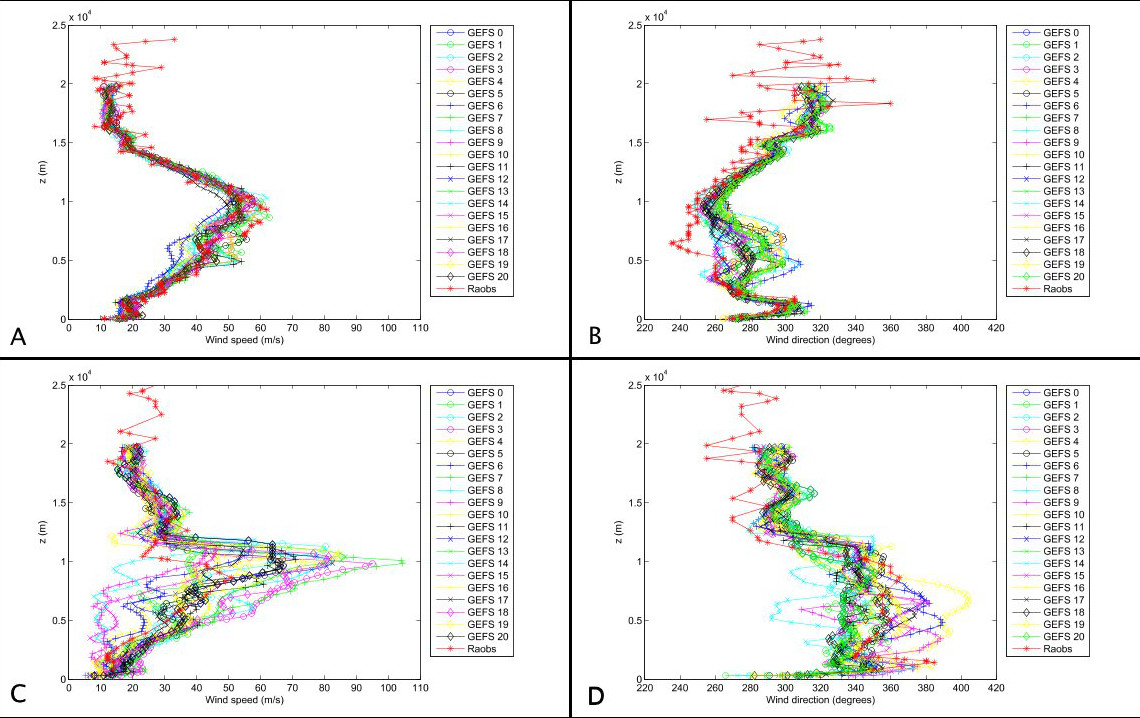
\includegraphics[width=\textwidth]{../figs/raob_compare.jpg}
 \caption{Comparison of wind speed (m/s) and wind direction (degrees) from radiosondes with those from GEFS and WRF multi-model output at (A and B), Praha station -- 00h forecast (C and D), and with multiphysics output at Praha station -- 72h forecast.}
 \label{fig_sounds}
 \end{figure}
 
 
 \begin{figure}[H!]
 \noindent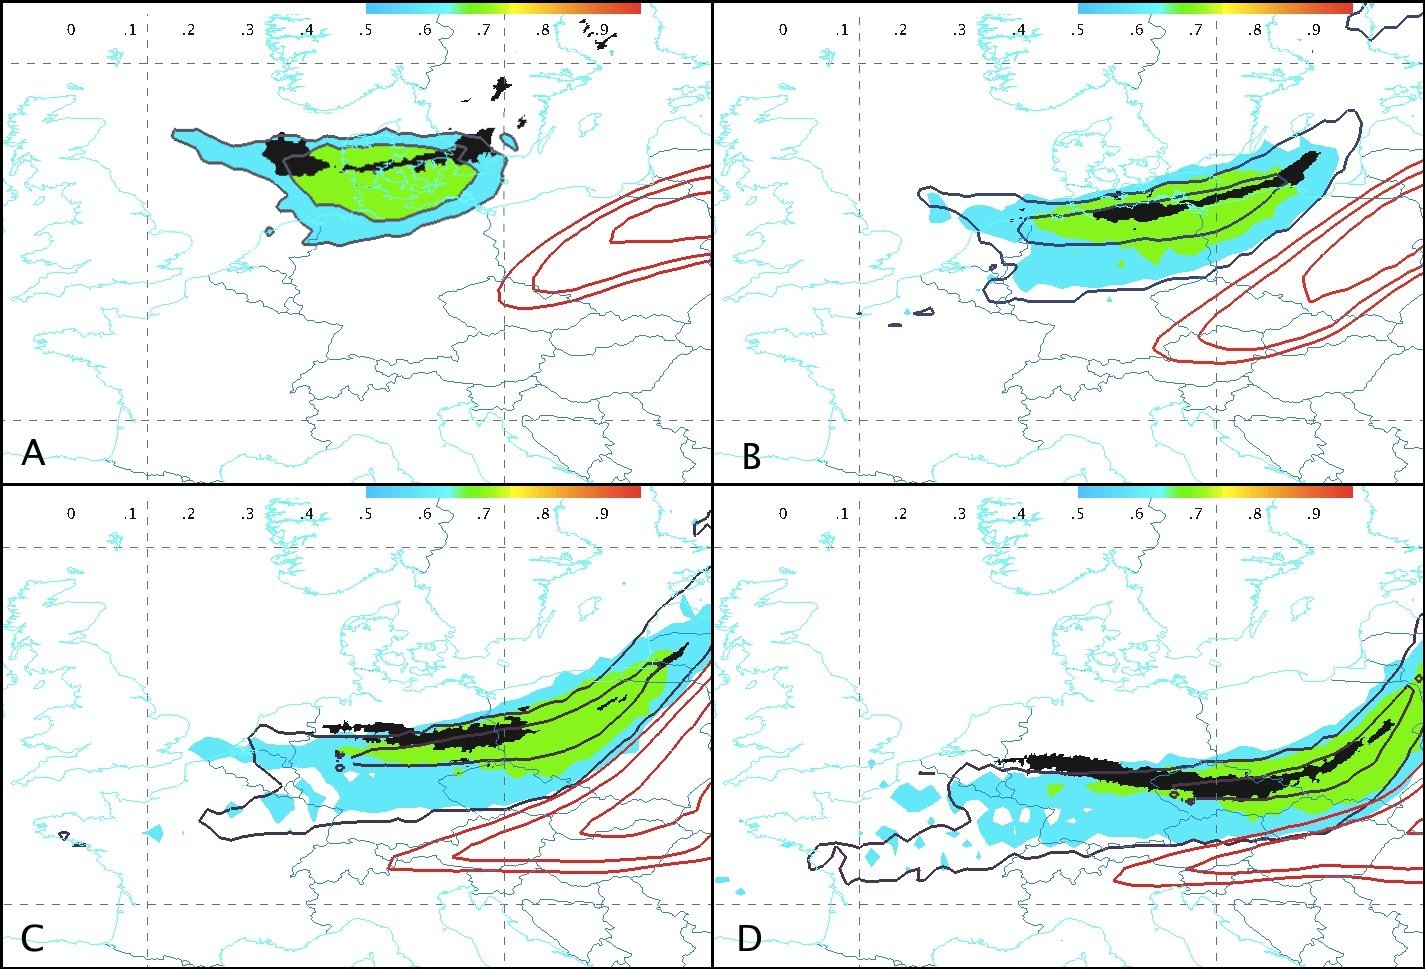
\includegraphics[width=\textwidth]{../figs/probabilityGeocat-2.jpg}
 \caption{Average probability of having airborne ash when accounting for source parameters only (color fill); source parameters and wind field variability - forecast starting 0000 UTC April 16 (black probability contour); source parameters and wind field variability -- forecast starting 0000 UTC April 14 (red probability contour), and corresponding satellite image (black fill), (A) 0000 UTC April 16, (B) 0006 UTC April 16, (C) 0012 UTC April 16, and (D) 0018 UTC April 16}.
 \label{fig_avg}
 \end{figure}

 
 \begin{figure}[H!]
 \centering
 \noindent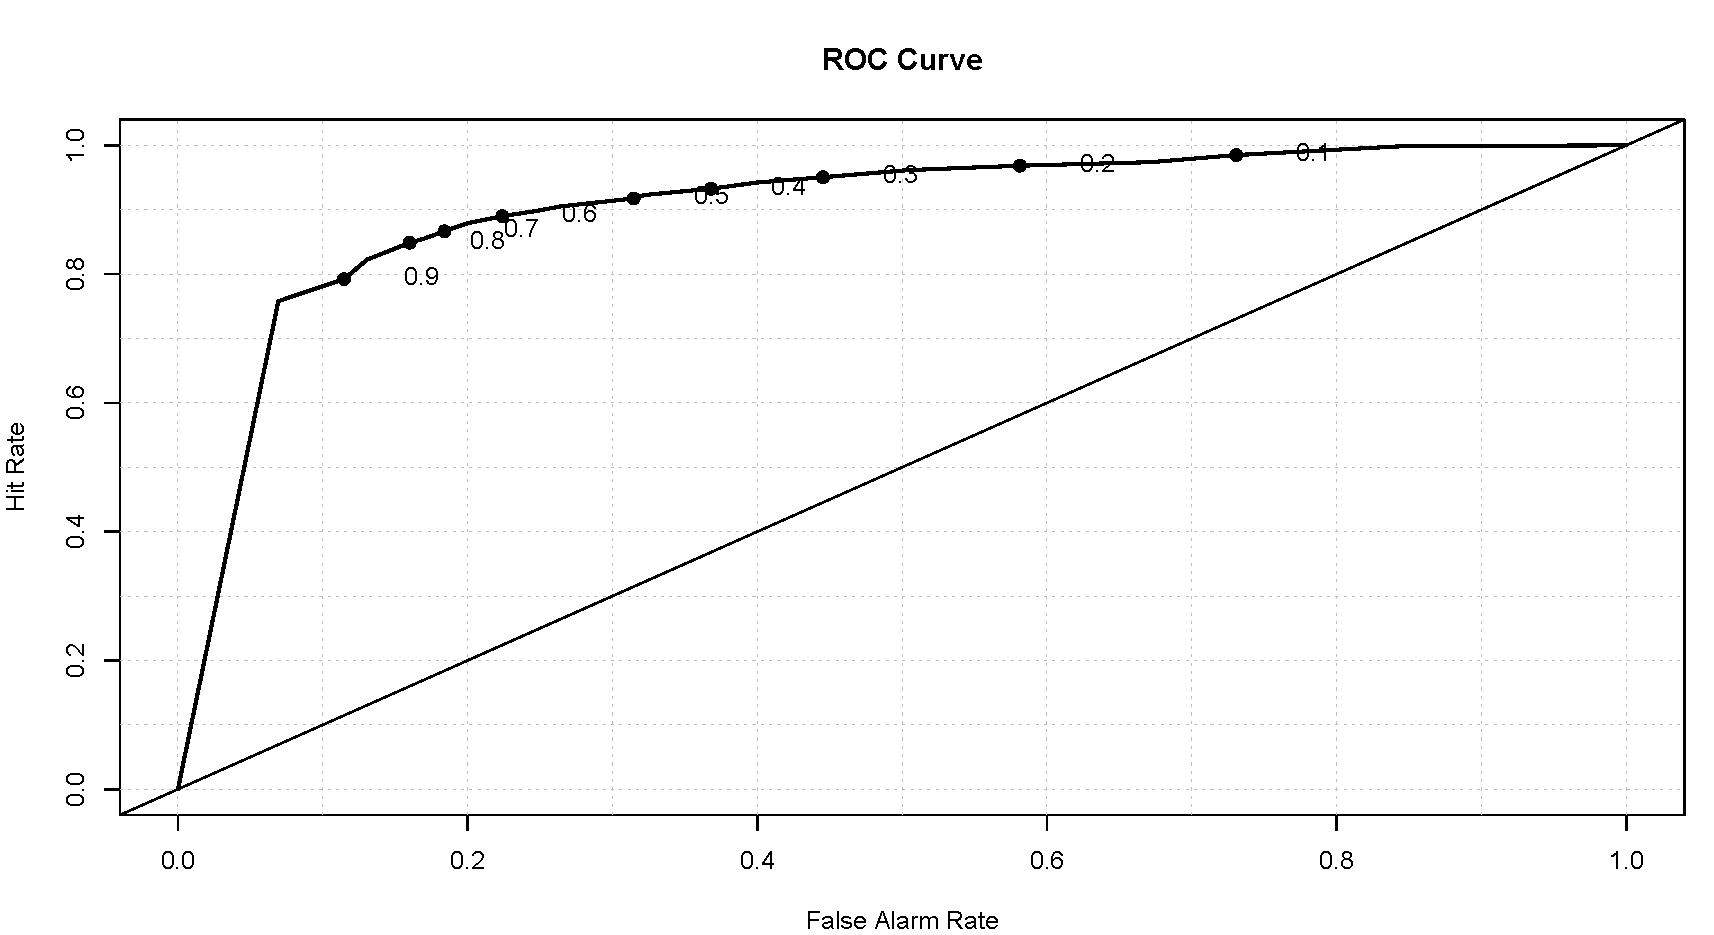
\includegraphics[width=\textwidth]{../figs/ROCplot_April16_06.pdf} (a) \\
  \noindent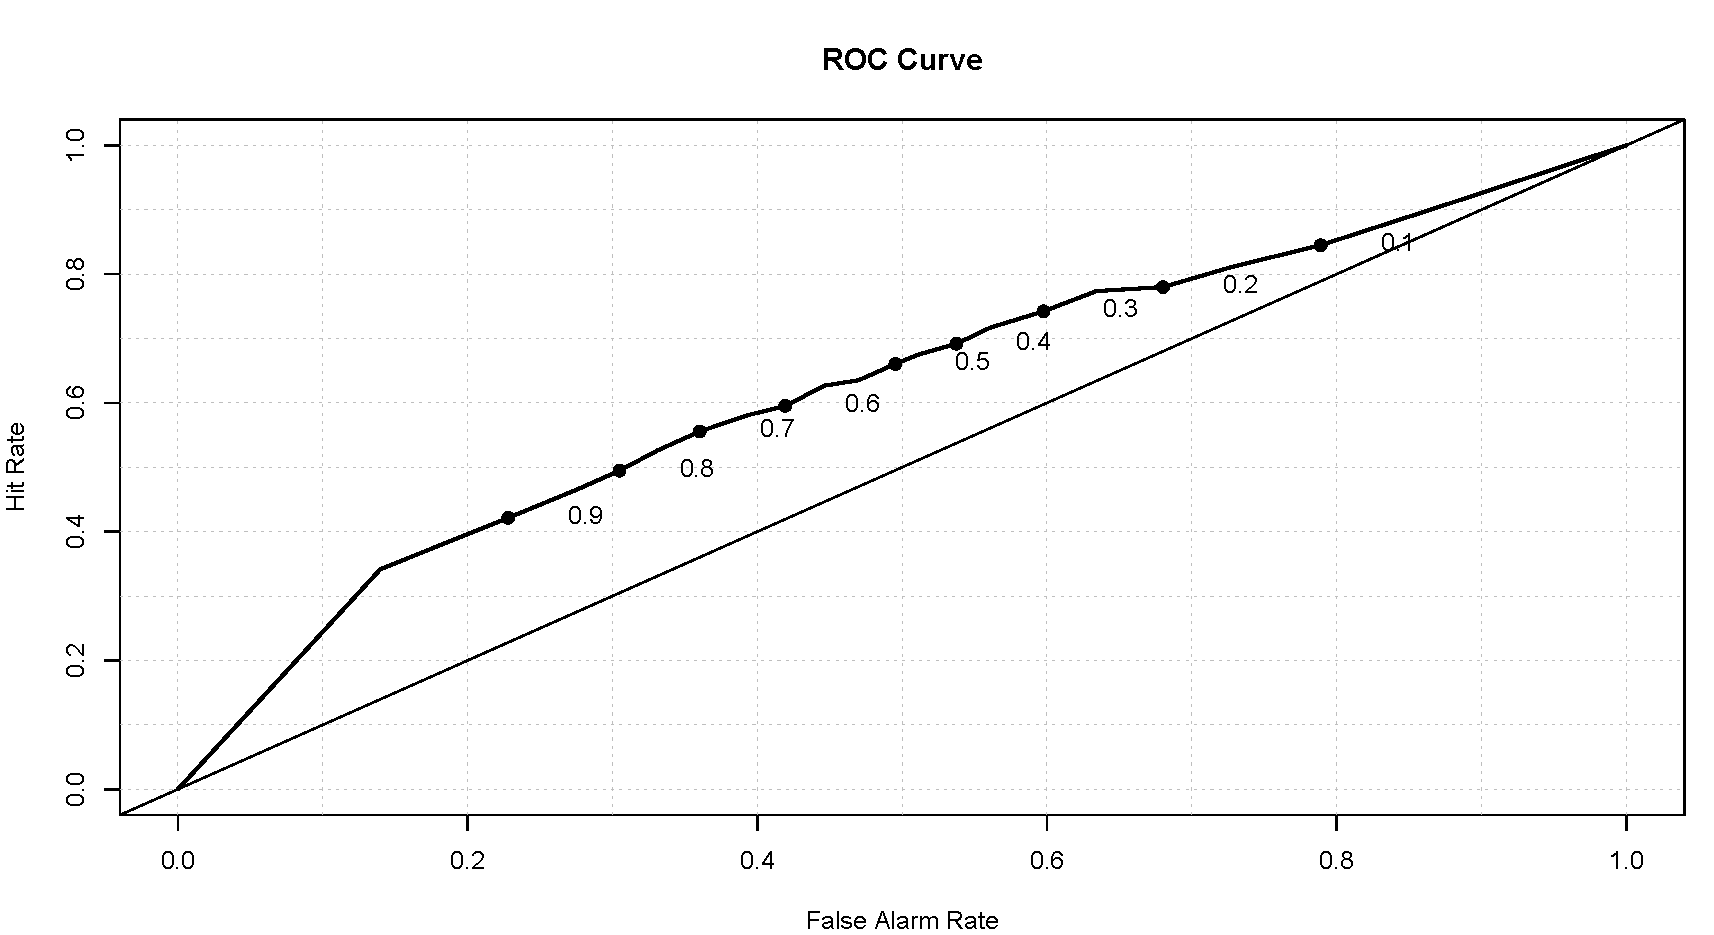
\includegraphics[width=\textwidth]{../figs/ROCplot_April16_06_from14.pdf} (b)
 \caption{Receiver Operating Characteristics (ROC) for maximum height of concentration exceeding $10^{-10}$ for source parameters and wind field variability and source parameters only a) forecast starts 0006 UTC April 16  b) forecast start at 0006 UTC April 14.}
 \label{roc_curve}
 \end{figure}

 
 \begin{figure}[H!]
 \noindent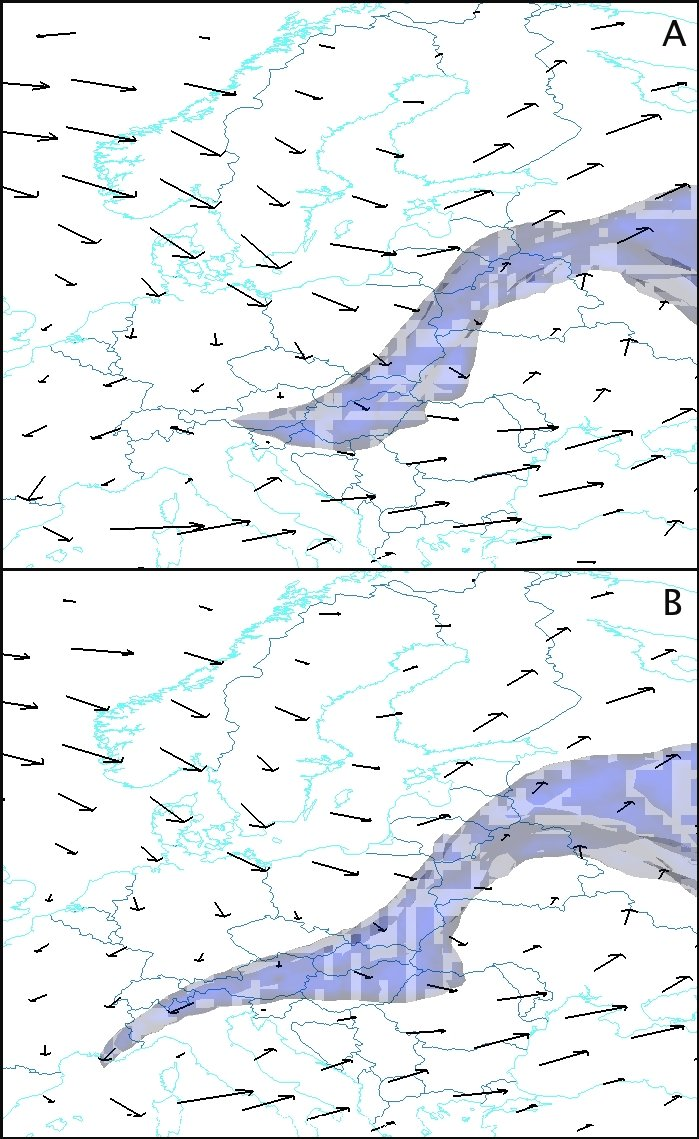
\includegraphics[width=0.7\textwidth]{../figs/skeb.jpg}
 \caption{(a) The 0005 UTC April 14 forecast starting 0000 UTC April 16 compared to the }
 \label{fig_skeb}
 \end{figure}
 

\end{document}

%%%%%%%%%%%%%%%%%%%%%%%%%%%%%%%%%%%%%%%%%%%%%%%%%%%%%%%%%%%%%%%

More Information and Advice:

%% ------------------------------------------------------------------------ %%
%
%  SECTION HEADS
%
%% ------------------------------------------------------------------------ %%

% Capitalize the first letter of each word (except for
% prepositions, conjunctions, and articles that are
% three or fewer letters).

% AGU follows standard outline style; therefore, there cannot be a section 1 without
% a section 2, or a section 2.3.1 without a section 2.3.2.
% Please make sure your section numbers are balanced.
% ---------------
% Level 1 head
%
% Use the \section{} command to identify level 1 heads;
% type the appropriate head wording between the curly
% brackets, as shown below.
%
%An example:
%\section{Level 1 Head: Introduction}
%
% ---------------
% Level 2 head
%
% Use the \subsection{} command to identify level 2 heads.
%An example:
%\subsection{Level 2 Head}
%
% ---------------
% Level 3 head
%
% Use the \subsubsection{} command to identify level 3 heads
%An example:
%\subsubsection{Level 3 Head}
%
%---------------
% Level 4 head
%
% Use the \subsubsubsection{} command to identify level 3 heads
% An example:
%\subsubsubsection{Level 4 Head} An example.
%
%% ------------------------------------------------------------------------ %%
%
%  IN-TEXT LISTS
%
%% ------------------------------------------------------------------------ %%
%
% Do not use bulleted lists; enumerated lists are okay.
% \begin{enumerate}
% \item
% \item
% \item
% \end{enumerate}
%
%% ------------------------------------------------------------------------ %%
%
%  EQUATIONS
%
%% ------------------------------------------------------------------------ %%

% Single-line equations are centered.
% Equation arrays will appear left-aligned.

Math coded inside display math mode \[ ...\]
 will not be numbered, e.g.,:
 \[ x^2=y^2 + z^2\]

 Math coded inside \begin{equation} and \end{equation} will
 be automatically numbered, e.g.,:
 \begin{equation}
 x^2=y^2 + z^2
 \end{equation}

% IF YOU HAVE MULTI-LINE EQUATIONS, PLEASE
% BREAK THE EQUATIONS INTO TWO OR MORE LINES
% OF SINGLE COLUMN WIDTH (20 pc, 8.3 cm)
% using double backslashes (\\).

% To create multiline equations, use the
% \begin{eqnarray} and \end{eqnarray} environment
% as demonstrated below.
\begin{eqnarray}
  x_{1} & = & (x - x_{0}) \cos \Theta \nonumber \\
        && + (y - y_{0}) \sin \Theta  \nonumber \\
  y_{1} & = & -(x - x_{0}) \sin \Theta \nonumber \\
        && + (y - y_{0}) \cos \Theta.
\end{eqnarray}

%If you don't want an equation number, use the star form:
%\begin{eqnarray*}...\end{eqnarray*}

% Break each line at a sign of operation
% (+, -, etc.) if possible, with the sign of operation
% on the new line.

% Indent second and subsequent lines to align with
% the first character following the equal sign on the
% first line.

% Use an \hspace{} command to insert horizontal space
% into your equation if necessary. Place an appropriate
% unit of measure between the curly braces, e.g.
% \hspace{1in}; you may have to experiment to achieve
% the correct amount of space.


%% ------------------------------------------------------------------------ %%
%
%  EQUATION NUMBERING: COUNTER
%
%% ------------------------------------------------------------------------ %%

% You may change equation numbering by resetting
% the equation counter or by explicitly numbering
% an equation.

% To explicitly number an equation, type \eqnum{}
% (with the desired number between the brackets)
% after the \begin{equation} or \begin{eqnarray}
% command.  The \eqnum{} command will affect only
% the equation it appears with; LaTeX will number
% any equations appearing later in the manuscript
% according to the equation counter.
%

% If you have a multiline equation that needs only
% one equation number, use a \nonumber command in
% front of the double backslashes (\\) as shown in
% the multiline equation above.

%% ------------------------------------------------------------------------ %%
%
%  LANDSCAPE/SIDEWAYS FIGURE AND TABLE EXAMPLES
%
%% ------------------------------------------------------------------------ %%
%
% For figures, add \usepackage{lscape} to the file and the landscape.sty style file
% to the paper folder.
%
% \begin{figure*}[p]
% \begin{landscapefigure*}
% Illustration here.
% \caption{caption here}
% \end{landscapefigure*}
% \end{figure*}
%
% For tables, add \usepackage{rotating} to the paper and add the rotating.sty file to the folder.
%
% AGU prefers the use of {sidewaystable} over {landscapetable} as it causes fewer problems.
%
% \begin{sidewaystable}
% \caption{}
% \begin{tabular}
% Table layout here.
% \end{tabular}
% \end{sidewaystable}
%
%
